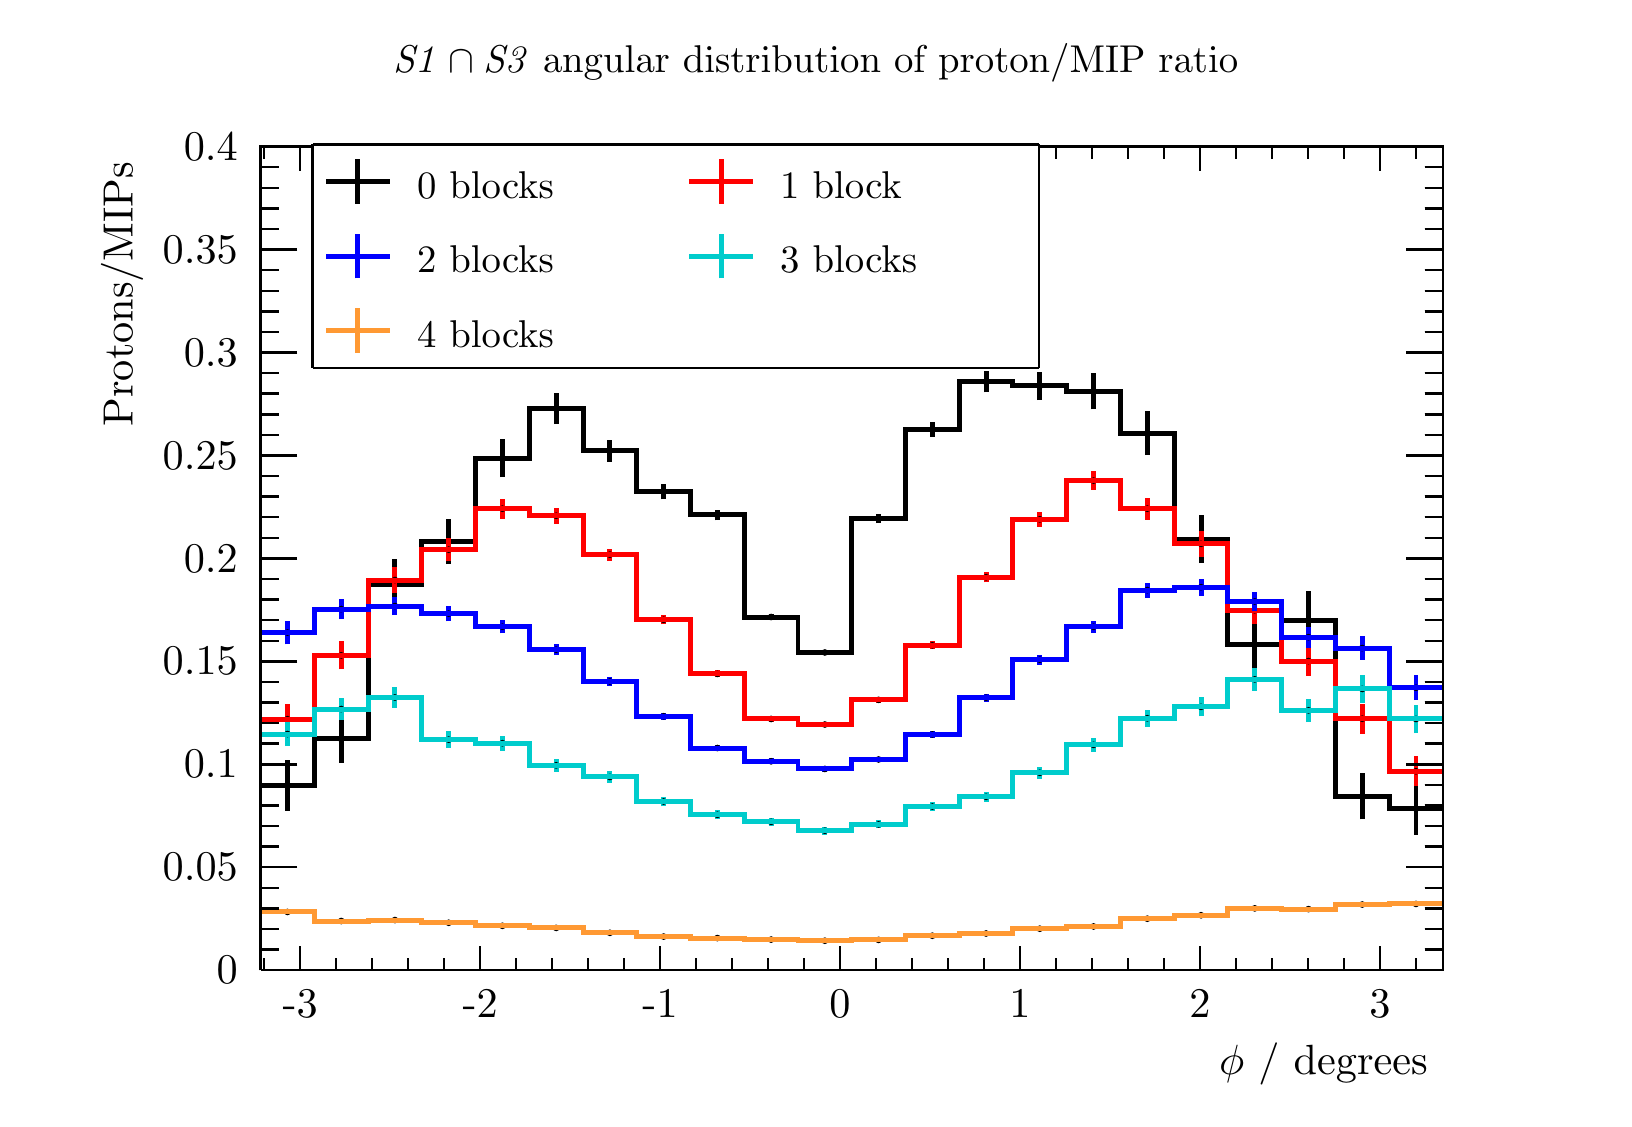
\begin{tikzpicture}
\pgfdeclareplotmark{cross} {
\pgfpathmoveto{\pgfpoint{-0.3\pgfplotmarksize}{\pgfplotmarksize}}
\pgfpathlineto{\pgfpoint{+0.3\pgfplotmarksize}{\pgfplotmarksize}}
\pgfpathlineto{\pgfpoint{+0.3\pgfplotmarksize}{0.3\pgfplotmarksize}}
\pgfpathlineto{\pgfpoint{+1\pgfplotmarksize}{0.3\pgfplotmarksize}}
\pgfpathlineto{\pgfpoint{+1\pgfplotmarksize}{-0.3\pgfplotmarksize}}
\pgfpathlineto{\pgfpoint{+0.3\pgfplotmarksize}{-0.3\pgfplotmarksize}}
\pgfpathlineto{\pgfpoint{+0.3\pgfplotmarksize}{-1.\pgfplotmarksize}}
\pgfpathlineto{\pgfpoint{-0.3\pgfplotmarksize}{-1.\pgfplotmarksize}}
\pgfpathlineto{\pgfpoint{-0.3\pgfplotmarksize}{-0.3\pgfplotmarksize}}
\pgfpathlineto{\pgfpoint{-1.\pgfplotmarksize}{-0.3\pgfplotmarksize}}
\pgfpathlineto{\pgfpoint{-1.\pgfplotmarksize}{0.3\pgfplotmarksize}}
\pgfpathlineto{\pgfpoint{-0.3\pgfplotmarksize}{0.3\pgfplotmarksize}}
\pgfpathclose
\pgfusepathqstroke
}
\pgfdeclareplotmark{cross*} {
\pgfpathmoveto{\pgfpoint{-0.3\pgfplotmarksize}{\pgfplotmarksize}}
\pgfpathlineto{\pgfpoint{+0.3\pgfplotmarksize}{\pgfplotmarksize}}
\pgfpathlineto{\pgfpoint{+0.3\pgfplotmarksize}{0.3\pgfplotmarksize}}
\pgfpathlineto{\pgfpoint{+1\pgfplotmarksize}{0.3\pgfplotmarksize}}
\pgfpathlineto{\pgfpoint{+1\pgfplotmarksize}{-0.3\pgfplotmarksize}}
\pgfpathlineto{\pgfpoint{+0.3\pgfplotmarksize}{-0.3\pgfplotmarksize}}
\pgfpathlineto{\pgfpoint{+0.3\pgfplotmarksize}{-1.\pgfplotmarksize}}
\pgfpathlineto{\pgfpoint{-0.3\pgfplotmarksize}{-1.\pgfplotmarksize}}
\pgfpathlineto{\pgfpoint{-0.3\pgfplotmarksize}{-0.3\pgfplotmarksize}}
\pgfpathlineto{\pgfpoint{-1.\pgfplotmarksize}{-0.3\pgfplotmarksize}}
\pgfpathlineto{\pgfpoint{-1.\pgfplotmarksize}{0.3\pgfplotmarksize}}
\pgfpathlineto{\pgfpoint{-0.3\pgfplotmarksize}{0.3\pgfplotmarksize}}
\pgfpathclose
\pgfusepathqfillstroke
}
\pgfdeclareplotmark{newstar} {
\pgfpathmoveto{\pgfqpoint{0pt}{\pgfplotmarksize}}
\pgfpathlineto{\pgfqpointpolar{44}{0.5\pgfplotmarksize}}
\pgfpathlineto{\pgfqpointpolar{18}{\pgfplotmarksize}}
\pgfpathlineto{\pgfqpointpolar{-20}{0.5\pgfplotmarksize}}
\pgfpathlineto{\pgfqpointpolar{-54}{\pgfplotmarksize}}
\pgfpathlineto{\pgfqpointpolar{-90}{0.5\pgfplotmarksize}}
\pgfpathlineto{\pgfqpointpolar{234}{\pgfplotmarksize}}
\pgfpathlineto{\pgfqpointpolar{198}{0.5\pgfplotmarksize}}
\pgfpathlineto{\pgfqpointpolar{162}{\pgfplotmarksize}}
\pgfpathlineto{\pgfqpointpolar{134}{0.5\pgfplotmarksize}}
\pgfpathclose
\pgfusepathqstroke
}
\pgfdeclareplotmark{newstar*} {
\pgfpathmoveto{\pgfqpoint{0pt}{\pgfplotmarksize}}
\pgfpathlineto{\pgfqpointpolar{44}{0.5\pgfplotmarksize}}
\pgfpathlineto{\pgfqpointpolar{18}{\pgfplotmarksize}}
\pgfpathlineto{\pgfqpointpolar{-20}{0.5\pgfplotmarksize}}
\pgfpathlineto{\pgfqpointpolar{-54}{\pgfplotmarksize}}
\pgfpathlineto{\pgfqpointpolar{-90}{0.5\pgfplotmarksize}}
\pgfpathlineto{\pgfqpointpolar{234}{\pgfplotmarksize}}
\pgfpathlineto{\pgfqpointpolar{198}{0.5\pgfplotmarksize}}
\pgfpathlineto{\pgfqpointpolar{162}{\pgfplotmarksize}}
\pgfpathlineto{\pgfqpointpolar{134}{0.5\pgfplotmarksize}}
\pgfpathclose
\pgfusepathqfillstroke
}
\definecolor{c}{rgb}{1,1,1};
\draw [color=c, fill=c] (0,0) rectangle (20,13.4957);
\draw [color=c, fill=c] (2.95129,1.53295) rectangle (17.9656,11.9914);
\definecolor{c}{rgb}{0,0,0};
\draw [c,line width=0.9] (2.95129,1.53295) -- (2.95129,11.9914) -- (17.9656,11.9914) -- (17.9656,1.53295) -- (2.95129,1.53295);
\definecolor{c}{rgb}{1,1,1};
\draw [color=c, fill=c] (2.95129,1.53295) rectangle (17.9656,11.9914);
\definecolor{c}{rgb}{0,0,0};
\draw [c,line width=0.9] (2.95129,1.53295) -- (2.95129,11.9914) -- (17.9656,11.9914) -- (17.9656,1.53295) -- (2.95129,1.53295);
\draw [c,line width=0.9] (2.95129,1.53295) -- (3.63376,1.53295) -- (3.63376,1.53295) -- (4.31623,1.53295) -- (4.31623,1.53295) -- (4.9987,1.53295) -- (4.9987,1.53295) -- (5.68117,1.53295) -- (5.68117,1.53295) -- (6.36364,1.53295) -- (6.36364,1.53295)
 -- (7.04611,1.53295) -- (7.04611,1.53295) -- (7.72858,1.53295) -- (7.72858,1.53295) -- (8.41104,1.53295) -- (8.41104,1.53295) -- (9.09351,1.53295) -- (9.09351,1.53295) -- (9.77598,1.53295) -- (9.77598,1.53295) -- (10.4585,1.53295) --
 (10.4585,1.53295) -- (11.1409,1.53295) -- (11.1409,1.53295) -- (11.8234,1.53295) -- (11.8234,1.53295) -- (12.5059,1.53295) -- (12.5059,1.53295) -- (13.1883,1.53295) -- (13.1883,1.53295) -- (13.8708,1.53295) -- (13.8708,1.53295) -- (14.5533,1.53295)
 -- (14.5533,1.53295) -- (15.2357,1.53295) -- (15.2357,1.53295) -- (15.9182,1.53295) -- (15.9182,1.53295) -- (16.6007,1.53295) -- (16.6007,1.53295) -- (17.2831,1.53295) -- (17.2831,1.53295) -- (17.9656,1.53295);
\draw [c,line width=0.9] (2.95129,1.53295) -- (17.9656,1.53295);
\draw [c,line width=0.9] (3.45405,1.83689) -- (3.45405,1.53295);
\draw [c,line width=0.9] (3.91111,1.68492) -- (3.91111,1.53295);
\draw [c,line width=0.9] (4.36817,1.68492) -- (4.36817,1.53295);
\draw [c,line width=0.9] (4.82522,1.68492) -- (4.82522,1.53295);
\draw [c,line width=0.9] (5.28228,1.68492) -- (5.28228,1.53295);
\draw [c,line width=0.9] (5.73934,1.83689) -- (5.73934,1.53295);
\draw [c,line width=0.9] (6.19639,1.68492) -- (6.19639,1.53295);
\draw [c,line width=0.9] (6.65345,1.68492) -- (6.65345,1.53295);
\draw [c,line width=0.9] (7.11051,1.68492) -- (7.11051,1.53295);
\draw [c,line width=0.9] (7.56757,1.68492) -- (7.56757,1.53295);
\draw [c,line width=0.9] (8.02462,1.83689) -- (8.02462,1.53295);
\draw [c,line width=0.9] (8.48168,1.68492) -- (8.48168,1.53295);
\draw [c,line width=0.9] (8.93874,1.68492) -- (8.93874,1.53295);
\draw [c,line width=0.9] (9.39579,1.68492) -- (9.39579,1.53295);
\draw [c,line width=0.9] (9.85285,1.68492) -- (9.85285,1.53295);
\draw [c,line width=0.9] (10.3099,1.83689) -- (10.3099,1.53295);
\draw [c,line width=0.9] (10.767,1.68492) -- (10.767,1.53295);
\draw [c,line width=0.9] (11.224,1.68492) -- (11.224,1.53295);
\draw [c,line width=0.9] (11.6811,1.68492) -- (11.6811,1.53295);
\draw [c,line width=0.9] (12.1381,1.68492) -- (12.1381,1.53295);
\draw [c,line width=0.9] (12.5952,1.83689) -- (12.5952,1.53295);
\draw [c,line width=0.9] (13.0523,1.68492) -- (13.0523,1.53295);
\draw [c,line width=0.9] (13.5093,1.68492) -- (13.5093,1.53295);
\draw [c,line width=0.9] (13.9664,1.68492) -- (13.9664,1.53295);
\draw [c,line width=0.9] (14.4234,1.68492) -- (14.4234,1.53295);
\draw [c,line width=0.9] (14.8805,1.83689) -- (14.8805,1.53295);
\draw [c,line width=0.9] (15.3375,1.68492) -- (15.3375,1.53295);
\draw [c,line width=0.9] (15.7946,1.68492) -- (15.7946,1.53295);
\draw [c,line width=0.9] (16.2517,1.68492) -- (16.2517,1.53295);
\draw [c,line width=0.9] (16.7087,1.68492) -- (16.7087,1.53295);
\draw [c,line width=0.9] (17.1658,1.83689) -- (17.1658,1.53295);
\draw [c,line width=0.9] (3.45405,1.83689) -- (3.45405,1.53295);
\draw [c,line width=0.9] (2.997,1.68492) -- (2.997,1.53295);
\draw [c,line width=0.9] (17.1658,1.83689) -- (17.1658,1.53295);
\draw [c,line width=0.9] (17.6228,1.68492) -- (17.6228,1.53295);
\draw [anchor=base] (3.45405,0.925645) node[scale=1.52731, color=c, rotate=0]{-3};
\draw [anchor=base] (5.73934,0.925645) node[scale=1.52731, color=c, rotate=0]{-2};
\draw [anchor=base] (8.02462,0.925645) node[scale=1.52731, color=c, rotate=0]{-1};
\draw [anchor=base] (10.3099,0.925645) node[scale=1.52731, color=c, rotate=0]{0};
\draw [anchor=base] (12.5952,0.925645) node[scale=1.52731, color=c, rotate=0]{1};
\draw [anchor=base] (14.8805,0.925645) node[scale=1.52731, color=c, rotate=0]{2};
\draw [anchor=base] (17.1658,0.925645) node[scale=1.52731, color=c, rotate=0]{3};
\draw [anchor= east] (17.9656,0.345329) node[scale=1.52731, color=c, rotate=0]{$ \phi$ / degrees};
\draw [c,line width=0.9] (2.95129,11.9914) -- (17.9656,11.9914);
\draw [c,line width=0.9] (3.45405,11.6875) -- (3.45405,11.9914);
\draw [c,line width=0.9] (3.91111,11.8394) -- (3.91111,11.9914);
\draw [c,line width=0.9] (4.36817,11.8394) -- (4.36817,11.9914);
\draw [c,line width=0.9] (4.82522,11.8394) -- (4.82522,11.9914);
\draw [c,line width=0.9] (5.28228,11.8394) -- (5.28228,11.9914);
\draw [c,line width=0.9] (5.73934,11.6875) -- (5.73934,11.9914);
\draw [c,line width=0.9] (6.19639,11.8394) -- (6.19639,11.9914);
\draw [c,line width=0.9] (6.65345,11.8394) -- (6.65345,11.9914);
\draw [c,line width=0.9] (7.11051,11.8394) -- (7.11051,11.9914);
\draw [c,line width=0.9] (7.56757,11.8394) -- (7.56757,11.9914);
\draw [c,line width=0.9] (8.02462,11.6875) -- (8.02462,11.9914);
\draw [c,line width=0.9] (8.48168,11.8394) -- (8.48168,11.9914);
\draw [c,line width=0.9] (8.93874,11.8394) -- (8.93874,11.9914);
\draw [c,line width=0.9] (9.39579,11.8394) -- (9.39579,11.9914);
\draw [c,line width=0.9] (9.85285,11.8394) -- (9.85285,11.9914);
\draw [c,line width=0.9] (10.3099,11.6875) -- (10.3099,11.9914);
\draw [c,line width=0.9] (10.767,11.8394) -- (10.767,11.9914);
\draw [c,line width=0.9] (11.224,11.8394) -- (11.224,11.9914);
\draw [c,line width=0.9] (11.6811,11.8394) -- (11.6811,11.9914);
\draw [c,line width=0.9] (12.1381,11.8394) -- (12.1381,11.9914);
\draw [c,line width=0.9] (12.5952,11.6875) -- (12.5952,11.9914);
\draw [c,line width=0.9] (13.0523,11.8394) -- (13.0523,11.9914);
\draw [c,line width=0.9] (13.5093,11.8394) -- (13.5093,11.9914);
\draw [c,line width=0.9] (13.9664,11.8394) -- (13.9664,11.9914);
\draw [c,line width=0.9] (14.4234,11.8394) -- (14.4234,11.9914);
\draw [c,line width=0.9] (14.8805,11.6875) -- (14.8805,11.9914);
\draw [c,line width=0.9] (15.3375,11.8394) -- (15.3375,11.9914);
\draw [c,line width=0.9] (15.7946,11.8394) -- (15.7946,11.9914);
\draw [c,line width=0.9] (16.2517,11.8394) -- (16.2517,11.9914);
\draw [c,line width=0.9] (16.7087,11.8394) -- (16.7087,11.9914);
\draw [c,line width=0.9] (17.1658,11.6875) -- (17.1658,11.9914);
\draw [c,line width=0.9] (3.45405,11.6875) -- (3.45405,11.9914);
\draw [c,line width=0.9] (2.997,11.8394) -- (2.997,11.9914);
\draw [c,line width=0.9] (17.1658,11.6875) -- (17.1658,11.9914);
\draw [c,line width=0.9] (17.6228,11.8394) -- (17.6228,11.9914);
\draw [c,line width=0.9] (2.95129,1.53295) -- (2.95129,11.9914);
\draw [c,line width=0.9] (3.41626,1.53295) -- (2.95129,1.53295);
\draw [c,line width=0.9] (3.18377,1.79441) -- (2.95129,1.79441);
\draw [c,line width=0.9] (3.18377,2.05587) -- (2.95129,2.05587);
\draw [c,line width=0.9] (3.18377,2.31734) -- (2.95129,2.31734);
\draw [c,line width=0.9] (3.18377,2.5788) -- (2.95129,2.5788);
\draw [c,line width=0.9] (3.41626,2.84026) -- (2.95129,2.84026);
\draw [c,line width=0.9] (3.18377,3.10172) -- (2.95129,3.10172);
\draw [c,line width=0.9] (3.18377,3.36318) -- (2.95129,3.36318);
\draw [c,line width=0.9] (3.18377,3.62464) -- (2.95129,3.62464);
\draw [c,line width=0.9] (3.18377,3.8861) -- (2.95129,3.8861);
\draw [c,line width=0.9] (3.41626,4.14756) -- (2.95129,4.14756);
\draw [c,line width=0.9] (3.18377,4.40903) -- (2.95129,4.40903);
\draw [c,line width=0.9] (3.18377,4.67049) -- (2.95129,4.67049);
\draw [c,line width=0.9] (3.18377,4.93195) -- (2.95129,4.93195);
\draw [c,line width=0.9] (3.18377,5.19341) -- (2.95129,5.19341);
\draw [c,line width=0.9] (3.41626,5.45487) -- (2.95129,5.45487);
\draw [c,line width=0.9] (3.18377,5.71633) -- (2.95129,5.71633);
\draw [c,line width=0.9] (3.18377,5.97779) -- (2.95129,5.97779);
\draw [c,line width=0.9] (3.18377,6.23925) -- (2.95129,6.23925);
\draw [c,line width=0.9] (3.18377,6.50072) -- (2.95129,6.50072);
\draw [c,line width=0.9] (3.41626,6.76218) -- (2.95129,6.76218);
\draw [c,line width=0.9] (3.18377,7.02364) -- (2.95129,7.02364);
\draw [c,line width=0.9] (3.18377,7.2851) -- (2.95129,7.2851);
\draw [c,line width=0.9] (3.18377,7.54656) -- (2.95129,7.54656);
\draw [c,line width=0.9] (3.18377,7.80802) -- (2.95129,7.80802);
\draw [c,line width=0.9] (3.41626,8.06948) -- (2.95129,8.06948);
\draw [c,line width=0.9] (3.18377,8.33095) -- (2.95129,8.33095);
\draw [c,line width=0.9] (3.18377,8.59241) -- (2.95129,8.59241);
\draw [c,line width=0.9] (3.18377,8.85387) -- (2.95129,8.85387);
\draw [c,line width=0.9] (3.18377,9.11533) -- (2.95129,9.11533);
\draw [c,line width=0.9] (3.41626,9.37679) -- (2.95129,9.37679);
\draw [c,line width=0.9] (3.18377,9.63825) -- (2.95129,9.63825);
\draw [c,line width=0.9] (3.18377,9.89971) -- (2.95129,9.89971);
\draw [c,line width=0.9] (3.18377,10.1612) -- (2.95129,10.1612);
\draw [c,line width=0.9] (3.18377,10.4226) -- (2.95129,10.4226);
\draw [c,line width=0.9] (3.41626,10.6841) -- (2.95129,10.6841);
\draw [c,line width=0.9] (3.18377,10.9456) -- (2.95129,10.9456);
\draw [c,line width=0.9] (3.18377,11.207) -- (2.95129,11.207);
\draw [c,line width=0.9] (3.18377,11.4685) -- (2.95129,11.4685);
\draw [c,line width=0.9] (3.18377,11.7299) -- (2.95129,11.7299);
\draw [c,line width=0.9] (3.41626,11.9914) -- (2.95129,11.9914);
\draw [anchor= east] (2.85129,1.53295) node[scale=1.52731, color=c, rotate=0]{0};
\draw [anchor= east] (2.85129,2.84026) node[scale=1.52731, color=c, rotate=0]{0.05};
\draw [anchor= east] (2.85129,4.14756) node[scale=1.52731, color=c, rotate=0]{0.1};
\draw [anchor= east] (2.85129,5.45487) node[scale=1.52731, color=c, rotate=0]{0.15};
\draw [anchor= east] (2.85129,6.76218) node[scale=1.52731, color=c, rotate=0]{0.2};
\draw [anchor= east] (2.85129,8.06948) node[scale=1.52731, color=c, rotate=0]{0.25};
\draw [anchor= east] (2.85129,9.37679) node[scale=1.52731, color=c, rotate=0]{0.3};
\draw [anchor= east] (2.85129,10.6841) node[scale=1.52731, color=c, rotate=0]{0.35};
\draw [anchor= east] (2.85129,11.9914) node[scale=1.52731, color=c, rotate=0]{0.4};
\draw [anchor= east] (1.19129,11.9914) node[scale=1.52731, color=c, rotate=90]{  Protons/MIPs};
\draw [c,line width=0.9] (17.9656,1.53295) -- (17.9656,11.9914);
\draw [c,line width=0.9] (17.5006,1.53295) -- (17.9656,1.53295);
\draw [c,line width=0.9] (17.7331,1.79441) -- (17.9656,1.79441);
\draw [c,line width=0.9] (17.7331,2.05587) -- (17.9656,2.05587);
\draw [c,line width=0.9] (17.7331,2.31734) -- (17.9656,2.31734);
\draw [c,line width=0.9] (17.7331,2.5788) -- (17.9656,2.5788);
\draw [c,line width=0.9] (17.5006,2.84026) -- (17.9656,2.84026);
\draw [c,line width=0.9] (17.7331,3.10172) -- (17.9656,3.10172);
\draw [c,line width=0.9] (17.7331,3.36318) -- (17.9656,3.36318);
\draw [c,line width=0.9] (17.7331,3.62464) -- (17.9656,3.62464);
\draw [c,line width=0.9] (17.7331,3.8861) -- (17.9656,3.8861);
\draw [c,line width=0.9] (17.5006,4.14756) -- (17.9656,4.14756);
\draw [c,line width=0.9] (17.7331,4.40903) -- (17.9656,4.40903);
\draw [c,line width=0.9] (17.7331,4.67049) -- (17.9656,4.67049);
\draw [c,line width=0.9] (17.7331,4.93195) -- (17.9656,4.93195);
\draw [c,line width=0.9] (17.7331,5.19341) -- (17.9656,5.19341);
\draw [c,line width=0.9] (17.5006,5.45487) -- (17.9656,5.45487);
\draw [c,line width=0.9] (17.7331,5.71633) -- (17.9656,5.71633);
\draw [c,line width=0.9] (17.7331,5.97779) -- (17.9656,5.97779);
\draw [c,line width=0.9] (17.7331,6.23925) -- (17.9656,6.23925);
\draw [c,line width=0.9] (17.7331,6.50072) -- (17.9656,6.50072);
\draw [c,line width=0.9] (17.5006,6.76218) -- (17.9656,6.76218);
\draw [c,line width=0.9] (17.7331,7.02364) -- (17.9656,7.02364);
\draw [c,line width=0.9] (17.7331,7.2851) -- (17.9656,7.2851);
\draw [c,line width=0.9] (17.7331,7.54656) -- (17.9656,7.54656);
\draw [c,line width=0.9] (17.7331,7.80802) -- (17.9656,7.80802);
\draw [c,line width=0.9] (17.5006,8.06948) -- (17.9656,8.06948);
\draw [c,line width=0.9] (17.7331,8.33095) -- (17.9656,8.33095);
\draw [c,line width=0.9] (17.7331,8.59241) -- (17.9656,8.59241);
\draw [c,line width=0.9] (17.7331,8.85387) -- (17.9656,8.85387);
\draw [c,line width=0.9] (17.7331,9.11533) -- (17.9656,9.11533);
\draw [c,line width=0.9] (17.5006,9.37679) -- (17.9656,9.37679);
\draw [c,line width=0.9] (17.7331,9.63825) -- (17.9656,9.63825);
\draw [c,line width=0.9] (17.7331,9.89971) -- (17.9656,9.89971);
\draw [c,line width=0.9] (17.7331,10.1612) -- (17.9656,10.1612);
\draw [c,line width=0.9] (17.7331,10.4226) -- (17.9656,10.4226);
\draw [c,line width=0.9] (17.5006,10.6841) -- (17.9656,10.6841);
\draw [c,line width=0.9] (17.7331,10.9456) -- (17.9656,10.9456);
\draw [c,line width=0.9] (17.7331,11.207) -- (17.9656,11.207);
\draw [c,line width=0.9] (17.7331,11.4685) -- (17.9656,11.4685);
\draw [c,line width=0.9] (17.7331,11.7299) -- (17.9656,11.7299);
\draw [c,line width=0.9] (17.5006,11.9914) -- (17.9656,11.9914);
\draw [c,line width=1.8] (3.29252,3.55953) -- (3.29252,3.88317);
\draw [c,line width=1.8] (3.29252,3.88317) -- (3.29252,4.20681);
\foreach \P in {(3.29252,3.88317)}{\draw[mark options={color=c,fill=c},mark size=2.402402pt,mark=*,mark size=1pt] plot coordinates {\P};}
\draw [c,line width=1.8] (3.97499,4.16432) -- (3.97499,4.46991);
\draw [c,line width=1.8] (3.97499,4.46991) -- (3.97499,4.77551);
\foreach \P in {(3.97499,4.46991)}{\draw[mark options={color=c,fill=c},mark size=2.402402pt,mark=*,mark size=1pt] plot coordinates {\P};}
\draw [c,line width=1.8] (4.65746,6.10421) -- (4.65746,6.42873);
\draw [c,line width=1.8] (4.65746,6.42873) -- (4.65746,6.75326);
\foreach \P in {(4.65746,6.42873)}{\draw[mark options={color=c,fill=c},mark size=2.402402pt,mark=*,mark size=1pt] plot coordinates {\P};}
\draw [c,line width=1.8] (5.33993,6.68868) -- (5.33993,6.97453);
\draw [c,line width=1.8] (5.33993,6.97453) -- (5.33993,7.26038);
\foreach \P in {(5.33993,6.97453)}{\draw[mark options={color=c,fill=c},mark size=2.402402pt,mark=*,mark size=1pt] plot coordinates {\P};}
\draw [c,line width=1.8] (6.0224,7.79316) -- (6.0224,8.03389);
\draw [c,line width=1.8] (6.0224,8.03389) -- (6.0224,8.27463);
\foreach \P in {(6.0224,8.03389)}{\draw[mark options={color=c,fill=c},mark size=2.402402pt,mark=*,mark size=1pt] plot coordinates {\P};}
\draw [c,line width=1.8] (6.70487,8.469) -- (6.70487,8.66305);
\draw [c,line width=1.8] (6.70487,8.66305) -- (6.70487,8.85711);
\foreach \P in {(6.70487,8.66305)}{\draw[mark options={color=c,fill=c},mark size=2.402402pt,mark=*,mark size=1pt] plot coordinates {\P};}
\draw [c,line width=1.8] (7.38734,7.9922) -- (7.38734,8.1309);
\draw [c,line width=1.8] (7.38734,8.1309) -- (7.38734,8.2696);
\foreach \P in {(7.38734,8.1309)}{\draw[mark options={color=c,fill=c},mark size=2.402402pt,mark=*,mark size=1pt] plot coordinates {\P};}
\draw [c,line width=1.8] (8.06981,7.51326) -- (8.06981,7.61035);
\draw [c,line width=1.8] (8.06981,7.61035) -- (8.06981,7.70743);
\foreach \P in {(8.06981,7.61035)}{\draw[mark options={color=c,fill=c},mark size=2.402402pt,mark=*,mark size=1pt] plot coordinates {\P};}
\draw [c,line width=1.8] (8.75228,7.24599) -- (8.75228,7.31399);
\draw [c,line width=1.8] (8.75228,7.31399) -- (8.75228,7.382);
\foreach \P in {(8.75228,7.31399)}{\draw[mark options={color=c,fill=c},mark size=2.402402pt,mark=*,mark size=1pt] plot coordinates {\P};}
\draw [c,line width=1.8] (9.43475,5.97993) -- (9.43475,6.01792);
\draw [c,line width=1.8] (9.43475,6.01792) -- (9.43475,6.0559);
\foreach \P in {(9.43475,6.01792)}{\draw[mark options={color=c,fill=c},mark size=2.402402pt,mark=*,mark size=1pt] plot coordinates {\P};}
\draw [c,line width=1.8] (10.1172,5.53526) -- (10.1172,5.56751);
\draw [c,line width=1.8] (10.1172,5.56751) -- (10.1172,5.59976);
\foreach \P in {(10.1172,5.56751)}{\draw[mark options={color=c,fill=c},mark size=2.402402pt,mark=*,mark size=1pt] plot coordinates {\P};}
\draw [c,line width=1.8] (10.7997,7.21049) -- (10.7997,7.26712);
\draw [c,line width=1.8] (10.7997,7.26712) -- (10.7997,7.32375);
\foreach \P in {(10.7997,7.26712)}{\draw[mark options={color=c,fill=c},mark size=2.402402pt,mark=*,mark size=1pt] plot coordinates {\P};}
\draw [c,line width=1.8] (11.4822,8.3056) -- (11.4822,8.39887);
\draw [c,line width=1.8] (11.4822,8.39887) -- (11.4822,8.49213);
\foreach \P in {(11.4822,8.39887)}{\draw[mark options={color=c,fill=c},mark size=2.402402pt,mark=*,mark size=1pt] plot coordinates {\P};}
\draw [c,line width=1.8] (12.1646,8.87157) -- (12.1646,9.00519);
\draw [c,line width=1.8] (12.1646,9.00519) -- (12.1646,9.1388);
\foreach \P in {(12.1646,9.00519)}{\draw[mark options={color=c,fill=c},mark size=2.402402pt,mark=*,mark size=1pt] plot coordinates {\P};}
\draw [c,line width=1.8] (12.8471,8.77134) -- (12.8471,8.95339);
\draw [c,line width=1.8] (12.8471,8.95339) -- (12.8471,9.13544);
\foreach \P in {(12.8471,8.95339)}{\draw[mark options={color=c,fill=c},mark size=2.402402pt,mark=*,mark size=1pt] plot coordinates {\P};}
\draw [c,line width=1.8] (13.5296,8.65581) -- (13.5296,8.88592);
\draw [c,line width=1.8] (13.5296,8.88592) -- (13.5296,9.11604);
\foreach \P in {(13.5296,8.88592)}{\draw[mark options={color=c,fill=c},mark size=2.402402pt,mark=*,mark size=1pt] plot coordinates {\P};}
\draw [c,line width=1.8] (14.212,8.07281) -- (14.212,8.35233);
\draw [c,line width=1.8] (14.212,8.35233) -- (14.212,8.63186);
\foreach \P in {(14.212,8.35233)}{\draw[mark options={color=c,fill=c},mark size=2.402402pt,mark=*,mark size=1pt] plot coordinates {\P};}
\draw [c,line width=1.8] (14.8945,6.70243) -- (14.8945,7.0079);
\draw [c,line width=1.8] (14.8945,7.0079) -- (14.8945,7.31337);
\foreach \P in {(14.8945,7.0079)}{\draw[mark options={color=c,fill=c},mark size=2.402402pt,mark=*,mark size=1pt] plot coordinates {\P};}
\draw [c,line width=1.8] (15.577,5.36523) -- (15.577,5.67119);
\draw [c,line width=1.8] (15.577,5.67119) -- (15.577,5.97715);
\foreach \P in {(15.577,5.67119)}{\draw[mark options={color=c,fill=c},mark size=2.402402pt,mark=*,mark size=1pt] plot coordinates {\P};}
\draw [c,line width=1.8] (16.2594,5.60828) -- (16.2594,5.97632);
\draw [c,line width=1.8] (16.2594,5.97632) -- (16.2594,6.34437);
\foreach \P in {(16.2594,5.97632)}{\draw[mark options={color=c,fill=c},mark size=2.402402pt,mark=*,mark size=1pt] plot coordinates {\P};}
\draw [c,line width=1.8] (16.9419,3.4472) -- (16.9419,3.74009);
\draw [c,line width=1.8] (16.9419,3.74009) -- (16.9419,4.03298);
\foreach \P in {(16.9419,3.74009)}{\draw[mark options={color=c,fill=c},mark size=2.402402pt,mark=*,mark size=1pt] plot coordinates {\P};}
\draw [c,line width=1.8] (17.6244,3.25182) -- (17.6244,3.58478);
\draw [c,line width=1.8] (17.6244,3.58478) -- (17.6244,3.91773);
\foreach \P in {(17.6244,3.58478)}{\draw[mark options={color=c,fill=c},mark size=2.402402pt,mark=*,mark size=1pt] plot coordinates {\P};}
\draw [c,line width=1.8] (2.95129,3.88317) -- (3.63376,3.88317) -- (3.63376,4.46991) -- (4.31623,4.46991) -- (4.31623,6.42873) -- (4.9987,6.42873) -- (4.9987,6.97453) -- (5.68117,6.97453) -- (5.68117,8.03389) -- (6.36364,8.03389) -- (6.36364,8.66305)
 -- (7.04611,8.66305) -- (7.04611,8.1309) -- (7.72858,8.1309) -- (7.72858,7.61035) -- (8.41104,7.61035) -- (8.41104,7.31399) -- (9.09351,7.31399) -- (9.09351,6.01792) -- (9.77598,6.01792) -- (9.77598,5.56751) -- (10.4585,5.56751) -- (10.4585,7.26712)
 -- (11.1409,7.26712) -- (11.1409,8.39887) -- (11.8234,8.39887) -- (11.8234,9.00519) -- (12.5059,9.00519) -- (12.5059,8.95339) -- (13.1883,8.95339) -- (13.1883,8.88592) -- (13.8708,8.88592) -- (13.8708,8.35233) -- (14.5533,8.35233) --
 (14.5533,7.0079) -- (15.2357,7.0079) -- (15.2357,5.67119) -- (15.9182,5.67119) -- (15.9182,5.97632) -- (16.6007,5.97632) -- (16.6007,3.74009) -- (17.2831,3.74009) -- (17.2831,3.58478) -- (17.9656,3.58478);
\definecolor{c}{rgb}{1,0,0};
\draw [c,line width=1.8] (3.29252,4.52886) -- (3.29252,4.71974);
\draw [c,line width=1.8] (3.29252,4.71974) -- (3.29252,4.91063);
\definecolor{c}{rgb}{0,0,0};
\foreach \P in {(3.29252,4.71974)}{\draw[mark options={color=c,fill=c},mark size=2.402402pt,mark=*,mark size=1pt] plot coordinates {\P};}
\definecolor{c}{rgb}{1,0,0};
\draw [c,line width=1.8] (3.97499,5.35208) -- (3.97499,5.53028);
\draw [c,line width=1.8] (3.97499,5.53028) -- (3.97499,5.70849);
\definecolor{c}{rgb}{0,0,0};
\foreach \P in {(3.97499,5.53028)}{\draw[mark options={color=c,fill=c},mark size=2.402402pt,mark=*,mark size=1pt] plot coordinates {\P};}
\definecolor{c}{rgb}{1,0,0};
\draw [c,line width=1.8] (4.65746,6.31708) -- (4.65746,6.48767);
\draw [c,line width=1.8] (4.65746,6.48767) -- (4.65746,6.65826);
\definecolor{c}{rgb}{0,0,0};
\foreach \P in {(4.65746,6.48767)}{\draw[mark options={color=c,fill=c},mark size=2.402402pt,mark=*,mark size=1pt] plot coordinates {\P};}
\definecolor{c}{rgb}{1,0,0};
\draw [c,line width=1.8] (5.33993,6.72532) -- (5.33993,6.87329);
\draw [c,line width=1.8] (5.33993,6.87329) -- (5.33993,7.02125);
\definecolor{c}{rgb}{0,0,0};
\foreach \P in {(5.33993,6.87329)}{\draw[mark options={color=c,fill=c},mark size=2.402402pt,mark=*,mark size=1pt] plot coordinates {\P};}
\definecolor{c}{rgb}{1,0,0};
\draw [c,line width=1.8] (6.0224,7.26622) -- (6.0224,7.39377);
\draw [c,line width=1.8] (6.0224,7.39377) -- (6.0224,7.52133);
\definecolor{c}{rgb}{0,0,0};
\foreach \P in {(6.0224,7.39377)}{\draw[mark options={color=c,fill=c},mark size=2.402402pt,mark=*,mark size=1pt] plot coordinates {\P};}
\definecolor{c}{rgb}{1,0,0};
\draw [c,line width=1.8] (6.70487,7.20219) -- (6.70487,7.30425);
\draw [c,line width=1.8] (6.70487,7.30425) -- (6.70487,7.40632);
\definecolor{c}{rgb}{0,0,0};
\foreach \P in {(6.70487,7.30425)}{\draw[mark options={color=c,fill=c},mark size=2.402402pt,mark=*,mark size=1pt] plot coordinates {\P};}
\definecolor{c}{rgb}{1,0,0};
\draw [c,line width=1.8] (7.38734,6.73337) -- (7.38734,6.81038);
\draw [c,line width=1.8] (7.38734,6.81038) -- (7.38734,6.8874);
\definecolor{c}{rgb}{0,0,0};
\foreach \P in {(7.38734,6.81038)}{\draw[mark options={color=c,fill=c},mark size=2.402402pt,mark=*,mark size=1pt] plot coordinates {\P};}
\definecolor{c}{rgb}{1,0,0};
\draw [c,line width=1.8] (8.06981,5.92607) -- (8.06981,5.98244);
\draw [c,line width=1.8] (8.06981,5.98244) -- (8.06981,6.03881);
\definecolor{c}{rgb}{0,0,0};
\foreach \P in {(8.06981,5.98244)}{\draw[mark options={color=c,fill=c},mark size=2.402402pt,mark=*,mark size=1pt] plot coordinates {\P};}
\definecolor{c}{rgb}{1,0,0};
\draw [c,line width=1.8] (8.75228,5.2515) -- (8.75228,5.29538);
\draw [c,line width=1.8] (8.75228,5.29538) -- (8.75228,5.33926);
\definecolor{c}{rgb}{0,0,0};
\foreach \P in {(8.75228,5.29538)}{\draw[mark options={color=c,fill=c},mark size=2.402402pt,mark=*,mark size=1pt] plot coordinates {\P};}
\definecolor{c}{rgb}{1,0,0};
\draw [c,line width=1.8] (9.43475,4.68796) -- (9.43475,4.72355);
\draw [c,line width=1.8] (9.43475,4.72355) -- (9.43475,4.75913);
\definecolor{c}{rgb}{0,0,0};
\foreach \P in {(9.43475,4.72355)}{\draw[mark options={color=c,fill=c},mark size=2.402402pt,mark=*,mark size=1pt] plot coordinates {\P};}
\definecolor{c}{rgb}{1,0,0};
\draw [c,line width=1.8] (10.1172,4.61827) -- (10.1172,4.6526);
\draw [c,line width=1.8] (10.1172,4.6526) -- (10.1172,4.68693);
\definecolor{c}{rgb}{0,0,0};
\foreach \P in {(10.1172,4.6526)}{\draw[mark options={color=c,fill=c},mark size=2.402402pt,mark=*,mark size=1pt] plot coordinates {\P};}
\definecolor{c}{rgb}{1,0,0};
\draw [c,line width=1.8] (10.7997,4.9273) -- (10.7997,4.9659);
\draw [c,line width=1.8] (10.7997,4.9659) -- (10.7997,5.00449);
\definecolor{c}{rgb}{0,0,0};
\foreach \P in {(10.7997,4.9659)}{\draw[mark options={color=c,fill=c},mark size=2.402402pt,mark=*,mark size=1pt] plot coordinates {\P};}
\definecolor{c}{rgb}{1,0,0};
\draw [c,line width=1.8] (11.4822,5.60952) -- (11.4822,5.65873);
\draw [c,line width=1.8] (11.4822,5.65873) -- (11.4822,5.70795);
\definecolor{c}{rgb}{0,0,0};
\foreach \P in {(11.4822,5.65873)}{\draw[mark options={color=c,fill=c},mark size=2.402402pt,mark=*,mark size=1pt] plot coordinates {\P};}
\definecolor{c}{rgb}{1,0,0};
\draw [c,line width=1.8] (12.1646,6.45653) -- (12.1646,6.52288);
\draw [c,line width=1.8] (12.1646,6.52288) -- (12.1646,6.58922);
\definecolor{c}{rgb}{0,0,0};
\foreach \P in {(12.1646,6.52288)}{\draw[mark options={color=c,fill=c},mark size=2.402402pt,mark=*,mark size=1pt] plot coordinates {\P};}
\definecolor{c}{rgb}{1,0,0};
\draw [c,line width=1.8] (12.8471,7.16675) -- (12.8471,7.25906);
\draw [c,line width=1.8] (12.8471,7.25906) -- (12.8471,7.35138);
\definecolor{c}{rgb}{0,0,0};
\foreach \P in {(12.8471,7.25906)}{\draw[mark options={color=c,fill=c},mark size=2.402402pt,mark=*,mark size=1pt] plot coordinates {\P};}
\definecolor{c}{rgb}{1,0,0};
\draw [c,line width=1.8] (13.5296,7.63243) -- (13.5296,7.75053);
\draw [c,line width=1.8] (13.5296,7.75053) -- (13.5296,7.86863);
\definecolor{c}{rgb}{0,0,0};
\foreach \P in {(13.5296,7.75053)}{\draw[mark options={color=c,fill=c},mark size=2.402402pt,mark=*,mark size=1pt] plot coordinates {\P};}
\definecolor{c}{rgb}{1,0,0};
\draw [c,line width=1.8] (14.212,7.25312) -- (14.212,7.39389);
\draw [c,line width=1.8] (14.212,7.39389) -- (14.212,7.53465);
\definecolor{c}{rgb}{0,0,0};
\foreach \P in {(14.212,7.39389)}{\draw[mark options={color=c,fill=c},mark size=2.402402pt,mark=*,mark size=1pt] plot coordinates {\P};}
\definecolor{c}{rgb}{1,0,0};
\draw [c,line width=1.8] (14.8945,6.785) -- (14.8945,6.94743);
\draw [c,line width=1.8] (14.8945,6.94743) -- (14.8945,7.10985);
\definecolor{c}{rgb}{0,0,0};
\foreach \P in {(14.8945,6.94743)}{\draw[mark options={color=c,fill=c},mark size=2.402402pt,mark=*,mark size=1pt] plot coordinates {\P};}
\definecolor{c}{rgb}{1,0,0};
\draw [c,line width=1.8] (15.577,5.92892) -- (15.577,6.10356);
\draw [c,line width=1.8] (15.577,6.10356) -- (15.577,6.2782);
\definecolor{c}{rgb}{0,0,0};
\foreach \P in {(15.577,6.10356)}{\draw[mark options={color=c,fill=c},mark size=2.402402pt,mark=*,mark size=1pt] plot coordinates {\P};}
\definecolor{c}{rgb}{1,0,0};
\draw [c,line width=1.8] (16.2594,5.27514) -- (16.2594,5.45833);
\draw [c,line width=1.8] (16.2594,5.45833) -- (16.2594,5.64153);
\definecolor{c}{rgb}{0,0,0};
\foreach \P in {(16.2594,5.45833)}{\draw[mark options={color=c,fill=c},mark size=2.402402pt,mark=*,mark size=1pt] plot coordinates {\P};}
\definecolor{c}{rgb}{1,0,0};
\draw [c,line width=1.8] (16.9419,4.53308) -- (16.9419,4.72611);
\draw [c,line width=1.8] (16.9419,4.72611) -- (16.9419,4.91913);
\definecolor{c}{rgb}{0,0,0};
\foreach \P in {(16.9419,4.72611)}{\draw[mark options={color=c,fill=c},mark size=2.402402pt,mark=*,mark size=1pt] plot coordinates {\P};}
\definecolor{c}{rgb}{1,0,0};
\draw [c,line width=1.8] (17.6244,3.86753) -- (17.6244,4.05929);
\draw [c,line width=1.8] (17.6244,4.05929) -- (17.6244,4.25105);
\definecolor{c}{rgb}{0,0,0};
\foreach \P in {(17.6244,4.05929)}{\draw[mark options={color=c,fill=c},mark size=2.402402pt,mark=*,mark size=1pt] plot coordinates {\P};}
\definecolor{c}{rgb}{1,0,0};
\draw [c,line width=1.8] (2.95129,4.71974) -- (3.63376,4.71974) -- (3.63376,5.53028) -- (4.31623,5.53028) -- (4.31623,6.48767) -- (4.9987,6.48767) -- (4.9987,6.87329) -- (5.68117,6.87329) -- (5.68117,7.39377) -- (6.36364,7.39377) -- (6.36364,7.30425)
 -- (7.04611,7.30425) -- (7.04611,6.81038) -- (7.72858,6.81038) -- (7.72858,5.98244) -- (8.41104,5.98244) -- (8.41104,5.29538) -- (9.09351,5.29538) -- (9.09351,4.72355) -- (9.77598,4.72355) -- (9.77598,4.6526) -- (10.4585,4.6526) -- (10.4585,4.9659)
 -- (11.1409,4.9659) -- (11.1409,5.65873) -- (11.8234,5.65873) -- (11.8234,6.52288) -- (12.5059,6.52288) -- (12.5059,7.25906) -- (13.1883,7.25906) -- (13.1883,7.75053) -- (13.8708,7.75053) -- (13.8708,7.39389) -- (14.5533,7.39389) --
 (14.5533,6.94743) -- (15.2357,6.94743) -- (15.2357,6.10356) -- (15.9182,6.10356) -- (15.9182,5.45833) -- (16.6007,5.45833) -- (16.6007,4.72611) -- (17.2831,4.72611) -- (17.2831,4.05929) -- (17.9656,4.05929);
\definecolor{c}{rgb}{0,0,1};
\draw [c,line width=1.8] (3.29252,5.67024) -- (3.29252,5.82025);
\draw [c,line width=1.8] (3.29252,5.82025) -- (3.29252,5.97026);
\definecolor{c}{rgb}{0,0,0};
\foreach \P in {(3.29252,5.82025)}{\draw[mark options={color=c,fill=c},mark size=2.402402pt,mark=*,mark size=1pt] plot coordinates {\P};}
\definecolor{c}{rgb}{0,0,1};
\draw [c,line width=1.8] (3.97499,5.9878) -- (3.97499,6.1185);
\draw [c,line width=1.8] (3.97499,6.1185) -- (3.97499,6.24921);
\definecolor{c}{rgb}{0,0,0};
\foreach \P in {(3.97499,6.1185)}{\draw[mark options={color=c,fill=c},mark size=2.402402pt,mark=*,mark size=1pt] plot coordinates {\P};}
\definecolor{c}{rgb}{0,0,1};
\draw [c,line width=1.8] (4.65746,6.04082) -- (4.65746,6.1567);
\draw [c,line width=1.8] (4.65746,6.1567) -- (4.65746,6.27258);
\definecolor{c}{rgb}{0,0,0};
\foreach \P in {(4.65746,6.1567)}{\draw[mark options={color=c,fill=c},mark size=2.402402pt,mark=*,mark size=1pt] plot coordinates {\P};}
\definecolor{c}{rgb}{0,0,1};
\draw [c,line width=1.8] (5.33993,5.96129) -- (5.33993,6.06052);
\draw [c,line width=1.8] (5.33993,6.06052) -- (5.33993,6.15976);
\definecolor{c}{rgb}{0,0,0};
\foreach \P in {(5.33993,6.06052)}{\draw[mark options={color=c,fill=c},mark size=2.402402pt,mark=*,mark size=1pt] plot coordinates {\P};}
\definecolor{c}{rgb}{0,0,1};
\draw [c,line width=1.8] (6.0224,5.81086) -- (6.0224,5.89445);
\draw [c,line width=1.8] (6.0224,5.89445) -- (6.0224,5.97804);
\definecolor{c}{rgb}{0,0,0};
\foreach \P in {(6.0224,5.89445)}{\draw[mark options={color=c,fill=c},mark size=2.402402pt,mark=*,mark size=1pt] plot coordinates {\P};}
\definecolor{c}{rgb}{0,0,1};
\draw [c,line width=1.8] (6.70487,5.53303) -- (6.70487,5.60316);
\draw [c,line width=1.8] (6.70487,5.60316) -- (6.70487,5.67329);
\definecolor{c}{rgb}{0,0,0};
\foreach \P in {(6.70487,5.60316)}{\draw[mark options={color=c,fill=c},mark size=2.402402pt,mark=*,mark size=1pt] plot coordinates {\P};}
\definecolor{c}{rgb}{0,0,1};
\draw [c,line width=1.8] (7.38734,5.14198) -- (7.38734,5.19945);
\draw [c,line width=1.8] (7.38734,5.19945) -- (7.38734,5.25691);
\definecolor{c}{rgb}{0,0,0};
\foreach \P in {(7.38734,5.19945)}{\draw[mark options={color=c,fill=c},mark size=2.402402pt,mark=*,mark size=1pt] plot coordinates {\P};}
\definecolor{c}{rgb}{0,0,1};
\draw [c,line width=1.8] (8.06981,4.71019) -- (8.06981,4.75708);
\draw [c,line width=1.8] (8.06981,4.75708) -- (8.06981,4.80396);
\definecolor{c}{rgb}{0,0,0};
\foreach \P in {(8.06981,4.75708)}{\draw[mark options={color=c,fill=c},mark size=2.402402pt,mark=*,mark size=1pt] plot coordinates {\P};}
\definecolor{c}{rgb}{0,0,1};
\draw [c,line width=1.8] (8.75228,4.3146) -- (8.75228,4.35429);
\draw [c,line width=1.8] (8.75228,4.35429) -- (8.75228,4.39398);
\definecolor{c}{rgb}{0,0,0};
\foreach \P in {(8.75228,4.35429)}{\draw[mark options={color=c,fill=c},mark size=2.402402pt,mark=*,mark size=1pt] plot coordinates {\P};}
\definecolor{c}{rgb}{0,0,1};
\draw [c,line width=1.8] (9.43475,4.14996) -- (9.43475,4.18562);
\draw [c,line width=1.8] (9.43475,4.18562) -- (9.43475,4.22128);
\definecolor{c}{rgb}{0,0,0};
\foreach \P in {(9.43475,4.18562)}{\draw[mark options={color=c,fill=c},mark size=2.402402pt,mark=*,mark size=1pt] plot coordinates {\P};}
\definecolor{c}{rgb}{0,0,1};
\draw [c,line width=1.8] (10.1172,4.0539) -- (10.1172,4.08874);
\draw [c,line width=1.8] (10.1172,4.08874) -- (10.1172,4.12358);
\definecolor{c}{rgb}{0,0,0};
\foreach \P in {(10.1172,4.08874)}{\draw[mark options={color=c,fill=c},mark size=2.402402pt,mark=*,mark size=1pt] plot coordinates {\P};}
\definecolor{c}{rgb}{0,0,1};
\draw [c,line width=1.8] (10.7997,4.17174) -- (10.7997,4.20873);
\draw [c,line width=1.8] (10.7997,4.20873) -- (10.7997,4.24572);
\definecolor{c}{rgb}{0,0,0};
\foreach \P in {(10.7997,4.20873)}{\draw[mark options={color=c,fill=c},mark size=2.402402pt,mark=*,mark size=1pt] plot coordinates {\P};}
\definecolor{c}{rgb}{0,0,1};
\draw [c,line width=1.8] (11.4822,4.48398) -- (11.4822,4.52662);
\draw [c,line width=1.8] (11.4822,4.52662) -- (11.4822,4.56925);
\definecolor{c}{rgb}{0,0,0};
\foreach \P in {(11.4822,4.52662)}{\draw[mark options={color=c,fill=c},mark size=2.402402pt,mark=*,mark size=1pt] plot coordinates {\P};}
\definecolor{c}{rgb}{0,0,1};
\draw [c,line width=1.8] (12.1646,4.94157) -- (12.1646,4.99305);
\draw [c,line width=1.8] (12.1646,4.99305) -- (12.1646,5.04452);
\definecolor{c}{rgb}{0,0,0};
\foreach \P in {(12.1646,4.99305)}{\draw[mark options={color=c,fill=c},mark size=2.402402pt,mark=*,mark size=1pt] plot coordinates {\P};}
\definecolor{c}{rgb}{0,0,1};
\draw [c,line width=1.8] (12.8471,5.4113) -- (12.8471,5.47643);
\draw [c,line width=1.8] (12.8471,5.47643) -- (12.8471,5.54156);
\definecolor{c}{rgb}{0,0,0};
\foreach \P in {(12.8471,5.47643)}{\draw[mark options={color=c,fill=c},mark size=2.402402pt,mark=*,mark size=1pt] plot coordinates {\P};}
\definecolor{c}{rgb}{0,0,1};
\draw [c,line width=1.8] (13.5296,5.81524) -- (13.5296,5.89423);
\draw [c,line width=1.8] (13.5296,5.89423) -- (13.5296,5.97322);
\definecolor{c}{rgb}{0,0,0};
\foreach \P in {(13.5296,5.89423)}{\draw[mark options={color=c,fill=c},mark size=2.402402pt,mark=*,mark size=1pt] plot coordinates {\P};}
\definecolor{c}{rgb}{0,0,1};
\draw [c,line width=1.8] (14.212,6.26482) -- (14.212,6.35996);
\draw [c,line width=1.8] (14.212,6.35996) -- (14.212,6.4551);
\definecolor{c}{rgb}{0,0,0};
\foreach \P in {(14.212,6.35996)}{\draw[mark options={color=c,fill=c},mark size=2.402402pt,mark=*,mark size=1pt] plot coordinates {\P};}
\definecolor{c}{rgb}{0,0,1};
\draw [c,line width=1.8] (14.8945,6.28798) -- (14.8945,6.39698);
\draw [c,line width=1.8] (14.8945,6.39698) -- (14.8945,6.50598);
\definecolor{c}{rgb}{0,0,0};
\foreach \P in {(14.8945,6.39698)}{\draw[mark options={color=c,fill=c},mark size=2.402402pt,mark=*,mark size=1pt] plot coordinates {\P};}
\definecolor{c}{rgb}{0,0,1};
\draw [c,line width=1.8] (15.577,6.09156) -- (15.577,6.21575);
\draw [c,line width=1.8] (15.577,6.21575) -- (15.577,6.33994);
\definecolor{c}{rgb}{0,0,0};
\foreach \P in {(15.577,6.21575)}{\draw[mark options={color=c,fill=c},mark size=2.402402pt,mark=*,mark size=1pt] plot coordinates {\P};}
\definecolor{c}{rgb}{0,0,1};
\draw [c,line width=1.8] (16.2594,5.62929) -- (16.2594,5.76214);
\draw [c,line width=1.8] (16.2594,5.76214) -- (16.2594,5.895);
\definecolor{c}{rgb}{0,0,0};
\foreach \P in {(16.2594,5.76214)}{\draw[mark options={color=c,fill=c},mark size=2.402402pt,mark=*,mark size=1pt] plot coordinates {\P};}
\definecolor{c}{rgb}{0,0,1};
\draw [c,line width=1.8] (16.9419,5.47315) -- (16.9419,5.6237);
\draw [c,line width=1.8] (16.9419,5.6237) -- (16.9419,5.77425);
\definecolor{c}{rgb}{0,0,0};
\foreach \P in {(16.9419,5.6237)}{\draw[mark options={color=c,fill=c},mark size=2.402402pt,mark=*,mark size=1pt] plot coordinates {\P};}
\definecolor{c}{rgb}{0,0,1};
\draw [c,line width=1.8] (17.6244,4.96092) -- (17.6244,5.11903);
\draw [c,line width=1.8] (17.6244,5.11903) -- (17.6244,5.27715);
\definecolor{c}{rgb}{0,0,0};
\foreach \P in {(17.6244,5.11903)}{\draw[mark options={color=c,fill=c},mark size=2.402402pt,mark=*,mark size=1pt] plot coordinates {\P};}
\definecolor{c}{rgb}{0,0,1};
\draw [c,line width=1.8] (2.95129,5.82025) -- (3.63376,5.82025) -- (3.63376,6.1185) -- (4.31623,6.1185) -- (4.31623,6.1567) -- (4.9987,6.1567) -- (4.9987,6.06052) -- (5.68117,6.06052) -- (5.68117,5.89445) -- (6.36364,5.89445) -- (6.36364,5.60316) --
 (7.04611,5.60316) -- (7.04611,5.19945) -- (7.72858,5.19945) -- (7.72858,4.75708) -- (8.41104,4.75708) -- (8.41104,4.35429) -- (9.09351,4.35429) -- (9.09351,4.18562) -- (9.77598,4.18562) -- (9.77598,4.08874) -- (10.4585,4.08874) -- (10.4585,4.20873)
 -- (11.1409,4.20873) -- (11.1409,4.52662) -- (11.8234,4.52662) -- (11.8234,4.99305) -- (12.5059,4.99305) -- (12.5059,5.47643) -- (13.1883,5.47643) -- (13.1883,5.89423) -- (13.8708,5.89423) -- (13.8708,6.35996) -- (14.5533,6.35996) --
 (14.5533,6.39698) -- (15.2357,6.39698) -- (15.2357,6.21575) -- (15.9182,6.21575) -- (15.9182,5.76214) -- (16.6007,5.76214) -- (16.6007,5.6237) -- (17.2831,5.6237) -- (17.2831,5.11903) -- (17.9656,5.11903);
\definecolor{c}{rgb}{0,0.8,0.8};
\draw [c,line width=1.8] (3.29252,4.37785) -- (3.29252,4.53205);
\draw [c,line width=1.8] (3.29252,4.53205) -- (3.29252,4.68625);
\definecolor{c}{rgb}{0,0,0};
\foreach \P in {(3.29252,4.53205)}{\draw[mark options={color=c,fill=c},mark size=2.402402pt,mark=*,mark size=1pt] plot coordinates {\P};}
\definecolor{c}{rgb}{0,0.8,0.8};
\draw [c,line width=1.8] (3.97499,4.70844) -- (3.97499,4.84912);
\draw [c,line width=1.8] (3.97499,4.84912) -- (3.97499,4.9898);
\definecolor{c}{rgb}{0,0,0};
\foreach \P in {(3.97499,4.84912)}{\draw[mark options={color=c,fill=c},mark size=2.402402pt,mark=*,mark size=1pt] plot coordinates {\P};}
\definecolor{c}{rgb}{0,0.8,0.8};
\draw [c,line width=1.8] (4.65746,4.86352) -- (4.65746,4.99571);
\draw [c,line width=1.8] (4.65746,4.99571) -- (4.65746,5.1279);
\definecolor{c}{rgb}{0,0,0};
\foreach \P in {(4.65746,4.99571)}{\draw[mark options={color=c,fill=c},mark size=2.402402pt,mark=*,mark size=1pt] plot coordinates {\P};}
\definecolor{c}{rgb}{0,0.8,0.8};
\draw [c,line width=1.8] (5.33993,4.35191) -- (5.33993,4.46062);
\draw [c,line width=1.8] (5.33993,4.46062) -- (5.33993,4.56932);
\definecolor{c}{rgb}{0,0,0};
\foreach \P in {(5.33993,4.46062)}{\draw[mark options={color=c,fill=c},mark size=2.402402pt,mark=*,mark size=1pt] plot coordinates {\P};}
\definecolor{c}{rgb}{0,0.8,0.8};
\draw [c,line width=1.8] (6.0224,4.31841) -- (6.0224,4.41522);
\draw [c,line width=1.8] (6.0224,4.41522) -- (6.0224,4.51202);
\definecolor{c}{rgb}{0,0,0};
\foreach \P in {(6.0224,4.41522)}{\draw[mark options={color=c,fill=c},mark size=2.402402pt,mark=*,mark size=1pt] plot coordinates {\P};}
\definecolor{c}{rgb}{0,0.8,0.8};
\draw [c,line width=1.8] (6.70487,4.05209) -- (6.70487,4.13442);
\draw [c,line width=1.8] (6.70487,4.13442) -- (6.70487,4.21676);
\definecolor{c}{rgb}{0,0,0};
\foreach \P in {(6.70487,4.13442)}{\draw[mark options={color=c,fill=c},mark size=2.402402pt,mark=*,mark size=1pt] plot coordinates {\P};}
\definecolor{c}{rgb}{0,0.8,0.8};
\draw [c,line width=1.8] (7.38734,3.91401) -- (7.38734,3.98652);
\draw [c,line width=1.8] (7.38734,3.98652) -- (7.38734,4.05903);
\definecolor{c}{rgb}{0,0,0};
\foreach \P in {(7.38734,3.98652)}{\draw[mark options={color=c,fill=c},mark size=2.402402pt,mark=*,mark size=1pt] plot coordinates {\P};}
\definecolor{c}{rgb}{0,0.8,0.8};
\draw [c,line width=1.8] (8.06981,3.61419) -- (8.06981,3.67503);
\draw [c,line width=1.8] (8.06981,3.67503) -- (8.06981,3.73587);
\definecolor{c}{rgb}{0,0,0};
\foreach \P in {(8.06981,3.67503)}{\draw[mark options={color=c,fill=c},mark size=2.402402pt,mark=*,mark size=1pt] plot coordinates {\P};}
\definecolor{c}{rgb}{0,0.8,0.8};
\draw [c,line width=1.8] (8.75228,3.45179) -- (8.75228,3.50644);
\draw [c,line width=1.8] (8.75228,3.50644) -- (8.75228,3.56109);
\definecolor{c}{rgb}{0,0,0};
\foreach \P in {(8.75228,3.50644)}{\draw[mark options={color=c,fill=c},mark size=2.402402pt,mark=*,mark size=1pt] plot coordinates {\P};}
\definecolor{c}{rgb}{0,0.8,0.8};
\draw [c,line width=1.8] (9.43475,3.36622) -- (9.43475,3.41687);
\draw [c,line width=1.8] (9.43475,3.41687) -- (9.43475,3.46752);
\definecolor{c}{rgb}{0,0,0};
\foreach \P in {(9.43475,3.41687)}{\draw[mark options={color=c,fill=c},mark size=2.402402pt,mark=*,mark size=1pt] plot coordinates {\P};}
\definecolor{c}{rgb}{0,0.8,0.8};
\draw [c,line width=1.8] (10.1172,3.25475) -- (10.1172,3.30385);
\draw [c,line width=1.8] (10.1172,3.30385) -- (10.1172,3.35295);
\definecolor{c}{rgb}{0,0,0};
\foreach \P in {(10.1172,3.30385)}{\draw[mark options={color=c,fill=c},mark size=2.402402pt,mark=*,mark size=1pt] plot coordinates {\P};}
\definecolor{c}{rgb}{0,0.8,0.8};
\draw [c,line width=1.8] (10.7997,3.33319) -- (10.7997,3.38415);
\draw [c,line width=1.8] (10.7997,3.38415) -- (10.7997,3.4351);
\definecolor{c}{rgb}{0,0,0};
\foreach \P in {(10.7997,3.38415)}{\draw[mark options={color=c,fill=c},mark size=2.402402pt,mark=*,mark size=1pt] plot coordinates {\P};}
\definecolor{c}{rgb}{0,0.8,0.8};
\draw [c,line width=1.8] (11.4822,3.55314) -- (11.4822,3.61089);
\draw [c,line width=1.8] (11.4822,3.61089) -- (11.4822,3.66865);
\definecolor{c}{rgb}{0,0,0};
\foreach \P in {(11.4822,3.61089)}{\draw[mark options={color=c,fill=c},mark size=2.402402pt,mark=*,mark size=1pt] plot coordinates {\P};}
\definecolor{c}{rgb}{0,0.8,0.8};
\draw [c,line width=1.8] (12.1646,3.67062) -- (12.1646,3.73458);
\draw [c,line width=1.8] (12.1646,3.73458) -- (12.1646,3.79855);
\definecolor{c}{rgb}{0,0,0};
\foreach \P in {(12.1646,3.73458)}{\draw[mark options={color=c,fill=c},mark size=2.402402pt,mark=*,mark size=1pt] plot coordinates {\P};}
\definecolor{c}{rgb}{0,0.8,0.8};
\draw [c,line width=1.8] (12.8471,3.96243) -- (12.8471,4.03946);
\draw [c,line width=1.8] (12.8471,4.03946) -- (12.8471,4.11648);
\definecolor{c}{rgb}{0,0,0};
\foreach \P in {(12.8471,4.03946)}{\draw[mark options={color=c,fill=c},mark size=2.402402pt,mark=*,mark size=1pt] plot coordinates {\P};}
\definecolor{c}{rgb}{0,0.8,0.8};
\draw [c,line width=1.8] (13.5296,4.30422) -- (13.5296,4.39451);
\draw [c,line width=1.8] (13.5296,4.39451) -- (13.5296,4.4848);
\definecolor{c}{rgb}{0,0,0};
\foreach \P in {(13.5296,4.39451)}{\draw[mark options={color=c,fill=c},mark size=2.402402pt,mark=*,mark size=1pt] plot coordinates {\P};}
\definecolor{c}{rgb}{0,0.8,0.8};
\draw [c,line width=1.8] (14.212,4.62525) -- (14.212,4.73212);
\draw [c,line width=1.8] (14.212,4.73212) -- (14.212,4.839);
\definecolor{c}{rgb}{0,0,0};
\foreach \P in {(14.212,4.73212)}{\draw[mark options={color=c,fill=c},mark size=2.402402pt,mark=*,mark size=1pt] plot coordinates {\P};}
\definecolor{c}{rgb}{0,0.8,0.8};
\draw [c,line width=1.8] (14.8945,4.75458) -- (14.8945,4.87687);
\draw [c,line width=1.8] (14.8945,4.87687) -- (14.8945,4.99917);
\definecolor{c}{rgb}{0,0,0};
\foreach \P in {(14.8945,4.87687)}{\draw[mark options={color=c,fill=c},mark size=2.402402pt,mark=*,mark size=1pt] plot coordinates {\P};}
\definecolor{c}{rgb}{0,0.8,0.8};
\draw [c,line width=1.8] (15.577,5.08258) -- (15.577,5.22606);
\draw [c,line width=1.8] (15.577,5.22606) -- (15.577,5.36954);
\definecolor{c}{rgb}{0,0,0};
\foreach \P in {(15.577,5.22606)}{\draw[mark options={color=c,fill=c},mark size=2.402402pt,mark=*,mark size=1pt] plot coordinates {\P};}
\definecolor{c}{rgb}{0,0.8,0.8};
\draw [c,line width=1.8] (16.2594,4.68435) -- (16.2594,4.8327);
\draw [c,line width=1.8] (16.2594,4.8327) -- (16.2594,4.98105);
\definecolor{c}{rgb}{0,0,0};
\foreach \P in {(16.2594,4.8327)}{\draw[mark options={color=c,fill=c},mark size=2.402402pt,mark=*,mark size=1pt] plot coordinates {\P};}
\definecolor{c}{rgb}{0,0.8,0.8};
\draw [c,line width=1.8] (16.9419,4.92585) -- (16.9419,5.10491);
\draw [c,line width=1.8] (16.9419,5.10491) -- (16.9419,5.28398);
\definecolor{c}{rgb}{0,0,0};
\foreach \P in {(16.9419,5.10491)}{\draw[mark options={color=c,fill=c},mark size=2.402402pt,mark=*,mark size=1pt] plot coordinates {\P};}
\definecolor{c}{rgb}{0,0.8,0.8};
\draw [c,line width=1.8] (17.6244,4.54362) -- (17.6244,4.723);
\draw [c,line width=1.8] (17.6244,4.723) -- (17.6244,4.90237);
\definecolor{c}{rgb}{0,0,0};
\foreach \P in {(17.6244,4.723)}{\draw[mark options={color=c,fill=c},mark size=2.402402pt,mark=*,mark size=1pt] plot coordinates {\P};}
\definecolor{c}{rgb}{0,0.8,0.8};
\draw [c,line width=1.8] (2.95129,4.53205) -- (3.63376,4.53205) -- (3.63376,4.84912) -- (4.31623,4.84912) -- (4.31623,4.99571) -- (4.9987,4.99571) -- (4.9987,4.46062) -- (5.68117,4.46062) -- (5.68117,4.41522) -- (6.36364,4.41522) -- (6.36364,4.13442)
 -- (7.04611,4.13442) -- (7.04611,3.98652) -- (7.72858,3.98652) -- (7.72858,3.67503) -- (8.41104,3.67503) -- (8.41104,3.50644) -- (9.09351,3.50644) -- (9.09351,3.41687) -- (9.77598,3.41687) -- (9.77598,3.30385) -- (10.4585,3.30385) --
 (10.4585,3.38415) -- (11.1409,3.38415) -- (11.1409,3.61089) -- (11.8234,3.61089) -- (11.8234,3.73458) -- (12.5059,3.73458) -- (12.5059,4.03946) -- (13.1883,4.03946) -- (13.1883,4.39451) -- (13.8708,4.39451) -- (13.8708,4.73212) -- (14.5533,4.73212)
 -- (14.5533,4.87687) -- (15.2357,4.87687) -- (15.2357,5.22606) -- (15.9182,5.22606) -- (15.9182,4.8327) -- (16.6007,4.8327) -- (16.6007,5.10491) -- (17.2831,5.10491) -- (17.2831,4.723) -- (17.9656,4.723);
\definecolor{c}{rgb}{1,0.6,0.2};
\draw [c,line width=1.8] (3.29252,2.25776) -- (3.29252,2.27238);
\draw [c,line width=1.8] (3.29252,2.27238) -- (3.29252,2.28701);
\definecolor{c}{rgb}{0,0,0};
\foreach \P in {(3.29252,2.27238)}{\draw[mark options={color=c,fill=c},mark size=2.402402pt,mark=*,mark size=1pt] plot coordinates {\P};}
\definecolor{c}{rgb}{1,0.6,0.2};
\draw [c,line width=1.8] (3.97499,2.14522) -- (3.97499,2.15721);
\draw [c,line width=1.8] (3.97499,2.15721) -- (3.97499,2.1692);
\definecolor{c}{rgb}{0,0,0};
\foreach \P in {(3.97499,2.15721)}{\draw[mark options={color=c,fill=c},mark size=2.402402pt,mark=*,mark size=1pt] plot coordinates {\P};}
\definecolor{c}{rgb}{1,0.6,0.2};
\draw [c,line width=1.8] (4.65746,2.15832) -- (4.65746,2.16951);
\draw [c,line width=1.8] (4.65746,2.16951) -- (4.65746,2.18071);
\definecolor{c}{rgb}{0,0,0};
\foreach \P in {(4.65746,2.16951)}{\draw[mark options={color=c,fill=c},mark size=2.402402pt,mark=*,mark size=1pt] plot coordinates {\P};}
\definecolor{c}{rgb}{1,0.6,0.2};
\draw [c,line width=1.8] (5.33993,2.12502) -- (5.33993,2.13494);
\draw [c,line width=1.8] (5.33993,2.13494) -- (5.33993,2.14486);
\definecolor{c}{rgb}{0,0,0};
\foreach \P in {(5.33993,2.13494)}{\draw[mark options={color=c,fill=c},mark size=2.402402pt,mark=*,mark size=1pt] plot coordinates {\P};}
\definecolor{c}{rgb}{1,0.6,0.2};
\draw [c,line width=1.8] (6.0224,2.08778) -- (6.0224,2.09652);
\draw [c,line width=1.8] (6.0224,2.09652) -- (6.0224,2.10527);
\definecolor{c}{rgb}{0,0,0};
\foreach \P in {(6.0224,2.09652)}{\draw[mark options={color=c,fill=c},mark size=2.402402pt,mark=*,mark size=1pt] plot coordinates {\P};}
\definecolor{c}{rgb}{1,0.6,0.2};
\draw [c,line width=1.8] (6.70487,2.06177) -- (6.70487,2.06965);
\draw [c,line width=1.8] (6.70487,2.06965) -- (6.70487,2.07753);
\definecolor{c}{rgb}{0,0,0};
\foreach \P in {(6.70487,2.06965)}{\draw[mark options={color=c,fill=c},mark size=2.402402pt,mark=*,mark size=1pt] plot coordinates {\P};}
\definecolor{c}{rgb}{1,0.6,0.2};
\draw [c,line width=1.8] (7.38734,2.00038) -- (7.38734,2.00729);
\draw [c,line width=1.8] (7.38734,2.00729) -- (7.38734,2.0142);
\definecolor{c}{rgb}{0,0,0};
\foreach \P in {(7.38734,2.00729)}{\draw[mark options={color=c,fill=c},mark size=2.402402pt,mark=*,mark size=1pt] plot coordinates {\P};}
\definecolor{c}{rgb}{1,0.6,0.2};
\draw [c,line width=1.8] (8.06981,1.95359) -- (8.06981,1.95959);
\draw [c,line width=1.8] (8.06981,1.95959) -- (8.06981,1.96559);
\definecolor{c}{rgb}{0,0,0};
\foreach \P in {(8.06981,1.95959)}{\draw[mark options={color=c,fill=c},mark size=2.402402pt,mark=*,mark size=1pt] plot coordinates {\P};}
\definecolor{c}{rgb}{1,0.6,0.2};
\draw [c,line width=1.8] (8.75228,1.93488) -- (8.75228,1.94047);
\draw [c,line width=1.8] (8.75228,1.94047) -- (8.75228,1.94607);
\definecolor{c}{rgb}{0,0,0};
\foreach \P in {(8.75228,1.94047)}{\draw[mark options={color=c,fill=c},mark size=2.402402pt,mark=*,mark size=1pt] plot coordinates {\P};}
\definecolor{c}{rgb}{1,0.6,0.2};
\draw [c,line width=1.8] (9.43475,1.91615) -- (9.43475,1.92136);
\draw [c,line width=1.8] (9.43475,1.92136) -- (9.43475,1.92656);
\definecolor{c}{rgb}{0,0,0};
\foreach \P in {(9.43475,1.92136)}{\draw[mark options={color=c,fill=c},mark size=2.402402pt,mark=*,mark size=1pt] plot coordinates {\P};}
\definecolor{c}{rgb}{1,0.6,0.2};
\draw [c,line width=1.8] (10.1172,1.9018) -- (10.1172,1.90692);
\draw [c,line width=1.8] (10.1172,1.90692) -- (10.1172,1.91205);
\definecolor{c}{rgb}{0,0,0};
\foreach \P in {(10.1172,1.90692)}{\draw[mark options={color=c,fill=c},mark size=2.402402pt,mark=*,mark size=1pt] plot coordinates {\P};}
\definecolor{c}{rgb}{1,0.6,0.2};
\draw [c,line width=1.8] (10.7997,1.91224) -- (10.7997,1.91751);
\draw [c,line width=1.8] (10.7997,1.91751) -- (10.7997,1.92277);
\definecolor{c}{rgb}{0,0,0};
\foreach \P in {(10.7997,1.91751)}{\draw[mark options={color=c,fill=c},mark size=2.402402pt,mark=*,mark size=1pt] plot coordinates {\P};}
\definecolor{c}{rgb}{1,0.6,0.2};
\draw [c,line width=1.8] (11.4822,1.96473) -- (11.4822,1.97069);
\draw [c,line width=1.8] (11.4822,1.97069) -- (11.4822,1.97665);
\definecolor{c}{rgb}{0,0,0};
\foreach \P in {(11.4822,1.97069)}{\draw[mark options={color=c,fill=c},mark size=2.402402pt,mark=*,mark size=1pt] plot coordinates {\P};}
\definecolor{c}{rgb}{1,0.6,0.2};
\draw [c,line width=1.8] (12.1646,1.99224) -- (12.1646,1.99879);
\draw [c,line width=1.8] (12.1646,1.99879) -- (12.1646,2.00535);
\definecolor{c}{rgb}{0,0,0};
\foreach \P in {(12.1646,1.99879)}{\draw[mark options={color=c,fill=c},mark size=2.402402pt,mark=*,mark size=1pt] plot coordinates {\P};}
\definecolor{c}{rgb}{1,0.6,0.2};
\draw [c,line width=1.8] (12.8471,2.05189) -- (12.8471,2.05964);
\draw [c,line width=1.8] (12.8471,2.05964) -- (12.8471,2.06739);
\definecolor{c}{rgb}{0,0,0};
\foreach \P in {(12.8471,2.05964)}{\draw[mark options={color=c,fill=c},mark size=2.402402pt,mark=*,mark size=1pt] plot coordinates {\P};}
\definecolor{c}{rgb}{1,0.6,0.2};
\draw [c,line width=1.8] (13.5296,2.07949) -- (13.5296,2.08804);
\draw [c,line width=1.8] (13.5296,2.08804) -- (13.5296,2.0966);
\definecolor{c}{rgb}{0,0,0};
\foreach \P in {(13.5296,2.08804)}{\draw[mark options={color=c,fill=c},mark size=2.402402pt,mark=*,mark size=1pt] plot coordinates {\P};}
\definecolor{c}{rgb}{1,0.6,0.2};
\draw [c,line width=1.8] (14.212,2.17652) -- (14.212,2.18657);
\draw [c,line width=1.8] (14.212,2.18657) -- (14.212,2.19662);
\definecolor{c}{rgb}{0,0,0};
\foreach \P in {(14.212,2.18657)}{\draw[mark options={color=c,fill=c},mark size=2.402402pt,mark=*,mark size=1pt] plot coordinates {\P};}
\definecolor{c}{rgb}{1,0.6,0.2};
\draw [c,line width=1.8] (14.8945,2.21922) -- (14.8945,2.2305);
\draw [c,line width=1.8] (14.8945,2.2305) -- (14.8945,2.24178);
\definecolor{c}{rgb}{0,0,0};
\foreach \P in {(14.8945,2.2305)}{\draw[mark options={color=c,fill=c},mark size=2.402402pt,mark=*,mark size=1pt] plot coordinates {\P};}
\definecolor{c}{rgb}{1,0.6,0.2};
\draw [c,line width=1.8] (15.577,2.30447) -- (15.577,2.31778);
\draw [c,line width=1.8] (15.577,2.31778) -- (15.577,2.3311);
\definecolor{c}{rgb}{0,0,0};
\foreach \P in {(15.577,2.31778)}{\draw[mark options={color=c,fill=c},mark size=2.402402pt,mark=*,mark size=1pt] plot coordinates {\P};}
\definecolor{c}{rgb}{1,0.6,0.2};
\draw [c,line width=1.8] (16.2594,2.29403) -- (16.2594,2.30815);
\draw [c,line width=1.8] (16.2594,2.30815) -- (16.2594,2.32227);
\definecolor{c}{rgb}{0,0,0};
\foreach \P in {(16.2594,2.30815)}{\draw[mark options={color=c,fill=c},mark size=2.402402pt,mark=*,mark size=1pt] plot coordinates {\P};}
\definecolor{c}{rgb}{1,0.6,0.2};
\draw [c,line width=1.8] (16.9419,2.35068) -- (16.9419,2.3667);
\draw [c,line width=1.8] (16.9419,2.3667) -- (16.9419,2.38273);
\definecolor{c}{rgb}{0,0,0};
\foreach \P in {(16.9419,2.3667)}{\draw[mark options={color=c,fill=c},mark size=2.402402pt,mark=*,mark size=1pt] plot coordinates {\P};}
\definecolor{c}{rgb}{1,0.6,0.2};
\draw [c,line width=1.8] (17.6244,2.35626) -- (17.6244,2.37437);
\draw [c,line width=1.8] (17.6244,2.37437) -- (17.6244,2.39248);
\definecolor{c}{rgb}{0,0,0};
\foreach \P in {(17.6244,2.37437)}{\draw[mark options={color=c,fill=c},mark size=2.402402pt,mark=*,mark size=1pt] plot coordinates {\P};}
\definecolor{c}{rgb}{1,0.6,0.2};
\draw [c,line width=1.8] (2.95129,2.27238) -- (3.63376,2.27238) -- (3.63376,2.15721) -- (4.31623,2.15721) -- (4.31623,2.16951) -- (4.9987,2.16951) -- (4.9987,2.13494) -- (5.68117,2.13494) -- (5.68117,2.09652) -- (6.36364,2.09652) -- (6.36364,2.06965)
 -- (7.04611,2.06965) -- (7.04611,2.00729) -- (7.72858,2.00729) -- (7.72858,1.95959) -- (8.41104,1.95959) -- (8.41104,1.94047) -- (9.09351,1.94047) -- (9.09351,1.92136) -- (9.77598,1.92136) -- (9.77598,1.90692) -- (10.4585,1.90692) --
 (10.4585,1.91751) -- (11.1409,1.91751) -- (11.1409,1.97069) -- (11.8234,1.97069) -- (11.8234,1.99879) -- (12.5059,1.99879) -- (12.5059,2.05964) -- (13.1883,2.05964) -- (13.1883,2.08804) -- (13.8708,2.08804) -- (13.8708,2.18657) -- (14.5533,2.18657)
 -- (14.5533,2.2305) -- (15.2357,2.2305) -- (15.2357,2.31778) -- (15.9182,2.31778) -- (15.9182,2.30815) -- (16.6007,2.30815) -- (16.6007,2.3667) -- (17.2831,2.3667) -- (17.2831,2.37437) -- (17.9656,2.37437);
\definecolor{c}{rgb}{0,0,0};
\draw [c,line width=0.9] (2.95129,1.53295) -- (17.9656,1.53295);
\draw [c,line width=0.9] (3.45405,1.83689) -- (3.45405,1.53295);
\draw [c,line width=0.9] (3.91111,1.68492) -- (3.91111,1.53295);
\draw [c,line width=0.9] (4.36817,1.68492) -- (4.36817,1.53295);
\draw [c,line width=0.9] (4.82522,1.68492) -- (4.82522,1.53295);
\draw [c,line width=0.9] (5.28228,1.68492) -- (5.28228,1.53295);
\draw [c,line width=0.9] (5.73934,1.83689) -- (5.73934,1.53295);
\draw [c,line width=0.9] (6.19639,1.68492) -- (6.19639,1.53295);
\draw [c,line width=0.9] (6.65345,1.68492) -- (6.65345,1.53295);
\draw [c,line width=0.9] (7.11051,1.68492) -- (7.11051,1.53295);
\draw [c,line width=0.9] (7.56757,1.68492) -- (7.56757,1.53295);
\draw [c,line width=0.9] (8.02462,1.83689) -- (8.02462,1.53295);
\draw [c,line width=0.9] (8.48168,1.68492) -- (8.48168,1.53295);
\draw [c,line width=0.9] (8.93874,1.68492) -- (8.93874,1.53295);
\draw [c,line width=0.9] (9.39579,1.68492) -- (9.39579,1.53295);
\draw [c,line width=0.9] (9.85285,1.68492) -- (9.85285,1.53295);
\draw [c,line width=0.9] (10.3099,1.83689) -- (10.3099,1.53295);
\draw [c,line width=0.9] (10.767,1.68492) -- (10.767,1.53295);
\draw [c,line width=0.9] (11.224,1.68492) -- (11.224,1.53295);
\draw [c,line width=0.9] (11.6811,1.68492) -- (11.6811,1.53295);
\draw [c,line width=0.9] (12.1381,1.68492) -- (12.1381,1.53295);
\draw [c,line width=0.9] (12.5952,1.83689) -- (12.5952,1.53295);
\draw [c,line width=0.9] (13.0523,1.68492) -- (13.0523,1.53295);
\draw [c,line width=0.9] (13.5093,1.68492) -- (13.5093,1.53295);
\draw [c,line width=0.9] (13.9664,1.68492) -- (13.9664,1.53295);
\draw [c,line width=0.9] (14.4234,1.68492) -- (14.4234,1.53295);
\draw [c,line width=0.9] (14.8805,1.83689) -- (14.8805,1.53295);
\draw [c,line width=0.9] (15.3375,1.68492) -- (15.3375,1.53295);
\draw [c,line width=0.9] (15.7946,1.68492) -- (15.7946,1.53295);
\draw [c,line width=0.9] (16.2517,1.68492) -- (16.2517,1.53295);
\draw [c,line width=0.9] (16.7087,1.68492) -- (16.7087,1.53295);
\draw [c,line width=0.9] (17.1658,1.83689) -- (17.1658,1.53295);
\draw [c,line width=0.9] (3.45405,1.83689) -- (3.45405,1.53295);
\draw [c,line width=0.9] (2.997,1.68492) -- (2.997,1.53295);
\draw [c,line width=0.9] (17.1658,1.83689) -- (17.1658,1.53295);
\draw [c,line width=0.9] (17.6228,1.68492) -- (17.6228,1.53295);
\draw [c,line width=0.9] (2.95129,11.9914) -- (17.9656,11.9914);
\draw [c,line width=0.9] (3.45405,11.6875) -- (3.45405,11.9914);
\draw [c,line width=0.9] (3.91111,11.8394) -- (3.91111,11.9914);
\draw [c,line width=0.9] (4.36817,11.8394) -- (4.36817,11.9914);
\draw [c,line width=0.9] (4.82522,11.8394) -- (4.82522,11.9914);
\draw [c,line width=0.9] (5.28228,11.8394) -- (5.28228,11.9914);
\draw [c,line width=0.9] (5.73934,11.6875) -- (5.73934,11.9914);
\draw [c,line width=0.9] (6.19639,11.8394) -- (6.19639,11.9914);
\draw [c,line width=0.9] (6.65345,11.8394) -- (6.65345,11.9914);
\draw [c,line width=0.9] (7.11051,11.8394) -- (7.11051,11.9914);
\draw [c,line width=0.9] (7.56757,11.8394) -- (7.56757,11.9914);
\draw [c,line width=0.9] (8.02462,11.6875) -- (8.02462,11.9914);
\draw [c,line width=0.9] (8.48168,11.8394) -- (8.48168,11.9914);
\draw [c,line width=0.9] (8.93874,11.8394) -- (8.93874,11.9914);
\draw [c,line width=0.9] (9.39579,11.8394) -- (9.39579,11.9914);
\draw [c,line width=0.9] (9.85285,11.8394) -- (9.85285,11.9914);
\draw [c,line width=0.9] (10.3099,11.6875) -- (10.3099,11.9914);
\draw [c,line width=0.9] (10.767,11.8394) -- (10.767,11.9914);
\draw [c,line width=0.9] (11.224,11.8394) -- (11.224,11.9914);
\draw [c,line width=0.9] (11.6811,11.8394) -- (11.6811,11.9914);
\draw [c,line width=0.9] (12.1381,11.8394) -- (12.1381,11.9914);
\draw [c,line width=0.9] (12.5952,11.6875) -- (12.5952,11.9914);
\draw [c,line width=0.9] (13.0523,11.8394) -- (13.0523,11.9914);
\draw [c,line width=0.9] (13.5093,11.8394) -- (13.5093,11.9914);
\draw [c,line width=0.9] (13.9664,11.8394) -- (13.9664,11.9914);
\draw [c,line width=0.9] (14.4234,11.8394) -- (14.4234,11.9914);
\draw [c,line width=0.9] (14.8805,11.6875) -- (14.8805,11.9914);
\draw [c,line width=0.9] (15.3375,11.8394) -- (15.3375,11.9914);
\draw [c,line width=0.9] (15.7946,11.8394) -- (15.7946,11.9914);
\draw [c,line width=0.9] (16.2517,11.8394) -- (16.2517,11.9914);
\draw [c,line width=0.9] (16.7087,11.8394) -- (16.7087,11.9914);
\draw [c,line width=0.9] (17.1658,11.6875) -- (17.1658,11.9914);
\draw [c,line width=0.9] (3.45405,11.6875) -- (3.45405,11.9914);
\draw [c,line width=0.9] (2.997,11.8394) -- (2.997,11.9914);
\draw [c,line width=0.9] (17.1658,11.6875) -- (17.1658,11.9914);
\draw [c,line width=0.9] (17.6228,11.8394) -- (17.6228,11.9914);
\draw [c,line width=0.9] (2.95129,1.53295) -- (2.95129,11.9914);
\draw [c,line width=0.9] (3.41626,1.53295) -- (2.95129,1.53295);
\draw [c,line width=0.9] (3.18377,1.79441) -- (2.95129,1.79441);
\draw [c,line width=0.9] (3.18377,2.05587) -- (2.95129,2.05587);
\draw [c,line width=0.9] (3.18377,2.31734) -- (2.95129,2.31734);
\draw [c,line width=0.9] (3.18377,2.5788) -- (2.95129,2.5788);
\draw [c,line width=0.9] (3.41626,2.84026) -- (2.95129,2.84026);
\draw [c,line width=0.9] (3.18377,3.10172) -- (2.95129,3.10172);
\draw [c,line width=0.9] (3.18377,3.36318) -- (2.95129,3.36318);
\draw [c,line width=0.9] (3.18377,3.62464) -- (2.95129,3.62464);
\draw [c,line width=0.9] (3.18377,3.8861) -- (2.95129,3.8861);
\draw [c,line width=0.9] (3.41626,4.14756) -- (2.95129,4.14756);
\draw [c,line width=0.9] (3.18377,4.40903) -- (2.95129,4.40903);
\draw [c,line width=0.9] (3.18377,4.67049) -- (2.95129,4.67049);
\draw [c,line width=0.9] (3.18377,4.93195) -- (2.95129,4.93195);
\draw [c,line width=0.9] (3.18377,5.19341) -- (2.95129,5.19341);
\draw [c,line width=0.9] (3.41626,5.45487) -- (2.95129,5.45487);
\draw [c,line width=0.9] (3.18377,5.71633) -- (2.95129,5.71633);
\draw [c,line width=0.9] (3.18377,5.97779) -- (2.95129,5.97779);
\draw [c,line width=0.9] (3.18377,6.23925) -- (2.95129,6.23925);
\draw [c,line width=0.9] (3.18377,6.50072) -- (2.95129,6.50072);
\draw [c,line width=0.9] (3.41626,6.76218) -- (2.95129,6.76218);
\draw [c,line width=0.9] (3.18377,7.02364) -- (2.95129,7.02364);
\draw [c,line width=0.9] (3.18377,7.2851) -- (2.95129,7.2851);
\draw [c,line width=0.9] (3.18377,7.54656) -- (2.95129,7.54656);
\draw [c,line width=0.9] (3.18377,7.80802) -- (2.95129,7.80802);
\draw [c,line width=0.9] (3.41626,8.06948) -- (2.95129,8.06948);
\draw [c,line width=0.9] (3.18377,8.33095) -- (2.95129,8.33095);
\draw [c,line width=0.9] (3.18377,8.59241) -- (2.95129,8.59241);
\draw [c,line width=0.9] (3.18377,8.85387) -- (2.95129,8.85387);
\draw [c,line width=0.9] (3.18377,9.11533) -- (2.95129,9.11533);
\draw [c,line width=0.9] (3.41626,9.37679) -- (2.95129,9.37679);
\draw [c,line width=0.9] (3.18377,9.63825) -- (2.95129,9.63825);
\draw [c,line width=0.9] (3.18377,9.89971) -- (2.95129,9.89971);
\draw [c,line width=0.9] (3.18377,10.1612) -- (2.95129,10.1612);
\draw [c,line width=0.9] (3.18377,10.4226) -- (2.95129,10.4226);
\draw [c,line width=0.9] (3.41626,10.6841) -- (2.95129,10.6841);
\draw [c,line width=0.9] (3.18377,10.9456) -- (2.95129,10.9456);
\draw [c,line width=0.9] (3.18377,11.207) -- (2.95129,11.207);
\draw [c,line width=0.9] (3.18377,11.4685) -- (2.95129,11.4685);
\draw [c,line width=0.9] (3.18377,11.7299) -- (2.95129,11.7299);
\draw [c,line width=0.9] (3.41626,11.9914) -- (2.95129,11.9914);
\draw [c,line width=0.9] (17.9656,1.53295) -- (17.9656,11.9914);
\draw [c,line width=0.9] (17.5006,1.53295) -- (17.9656,1.53295);
\draw [c,line width=0.9] (17.7331,1.79441) -- (17.9656,1.79441);
\draw [c,line width=0.9] (17.7331,2.05587) -- (17.9656,2.05587);
\draw [c,line width=0.9] (17.7331,2.31734) -- (17.9656,2.31734);
\draw [c,line width=0.9] (17.7331,2.5788) -- (17.9656,2.5788);
\draw [c,line width=0.9] (17.5006,2.84026) -- (17.9656,2.84026);
\draw [c,line width=0.9] (17.7331,3.10172) -- (17.9656,3.10172);
\draw [c,line width=0.9] (17.7331,3.36318) -- (17.9656,3.36318);
\draw [c,line width=0.9] (17.7331,3.62464) -- (17.9656,3.62464);
\draw [c,line width=0.9] (17.7331,3.8861) -- (17.9656,3.8861);
\draw [c,line width=0.9] (17.5006,4.14756) -- (17.9656,4.14756);
\draw [c,line width=0.9] (17.7331,4.40903) -- (17.9656,4.40903);
\draw [c,line width=0.9] (17.7331,4.67049) -- (17.9656,4.67049);
\draw [c,line width=0.9] (17.7331,4.93195) -- (17.9656,4.93195);
\draw [c,line width=0.9] (17.7331,5.19341) -- (17.9656,5.19341);
\draw [c,line width=0.9] (17.5006,5.45487) -- (17.9656,5.45487);
\draw [c,line width=0.9] (17.7331,5.71633) -- (17.9656,5.71633);
\draw [c,line width=0.9] (17.7331,5.97779) -- (17.9656,5.97779);
\draw [c,line width=0.9] (17.7331,6.23925) -- (17.9656,6.23925);
\draw [c,line width=0.9] (17.7331,6.50072) -- (17.9656,6.50072);
\draw [c,line width=0.9] (17.5006,6.76218) -- (17.9656,6.76218);
\draw [c,line width=0.9] (17.7331,7.02364) -- (17.9656,7.02364);
\draw [c,line width=0.9] (17.7331,7.2851) -- (17.9656,7.2851);
\draw [c,line width=0.9] (17.7331,7.54656) -- (17.9656,7.54656);
\draw [c,line width=0.9] (17.7331,7.80802) -- (17.9656,7.80802);
\draw [c,line width=0.9] (17.5006,8.06948) -- (17.9656,8.06948);
\draw [c,line width=0.9] (17.7331,8.33095) -- (17.9656,8.33095);
\draw [c,line width=0.9] (17.7331,8.59241) -- (17.9656,8.59241);
\draw [c,line width=0.9] (17.7331,8.85387) -- (17.9656,8.85387);
\draw [c,line width=0.9] (17.7331,9.11533) -- (17.9656,9.11533);
\draw [c,line width=0.9] (17.5006,9.37679) -- (17.9656,9.37679);
\draw [c,line width=0.9] (17.7331,9.63825) -- (17.9656,9.63825);
\draw [c,line width=0.9] (17.7331,9.89971) -- (17.9656,9.89971);
\draw [c,line width=0.9] (17.7331,10.1612) -- (17.9656,10.1612);
\draw [c,line width=0.9] (17.7331,10.4226) -- (17.9656,10.4226);
\draw [c,line width=0.9] (17.5006,10.6841) -- (17.9656,10.6841);
\draw [c,line width=0.9] (17.7331,10.9456) -- (17.9656,10.9456);
\draw [c,line width=0.9] (17.7331,11.207) -- (17.9656,11.207);
\draw [c,line width=0.9] (17.7331,11.4685) -- (17.9656,11.4685);
\draw [c,line width=0.9] (17.7331,11.7299) -- (17.9656,11.7299);
\draw [c,line width=0.9] (17.5006,11.9914) -- (17.9656,11.9914);
\definecolor{c}{rgb}{1,1,1};
\draw [color=c, fill=c] (2,12.686) rectangle (18,13.4282);
\definecolor{c}{rgb}{0,0,0};
\draw (10,13.0571) node[scale=1.40004, color=c, rotate=0]{$\mathit{S1} \cap \mathit{S3}$ angular distribution of proton/MIP ratio};
\definecolor{c}{rgb}{1,1,1};
\draw [color=c, fill=c] (3.61032,9.18338) rectangle (12.8367,12.0201);
\definecolor{c}{rgb}{0,0,0};
\draw [c,line width=0.9] (3.61032,9.18338) -- (12.8367,9.18338);
\draw [c,line width=0.9] (12.8367,9.18338) -- (12.8367,12.0201);
\draw [c,line width=0.9] (12.8367,12.0201) -- (3.61032,12.0201);
\draw [c,line width=0.9] (3.61032,12.0201) -- (3.61032,9.18338);
\draw [anchor=base west] (4.76361,11.3345) node[scale=1.40004, color=c, rotate=0]{0 blocks};
\draw [c,line width=1.8] (3.78331,11.5473) -- (4.59062,11.5473);
\draw [c,line width=1.8] (4.18696,11.2636) -- (4.18696,11.8309);
\draw [anchor=base west] (9.37679,11.3345) node[scale=1.40004, color=c, rotate=0]{1 block};
\definecolor{c}{rgb}{1,0,0};
\draw [c,line width=1.8] (8.39649,11.5473) -- (9.2038,11.5473);
\draw [c,line width=1.8] (8.80014,11.2636) -- (8.80014,11.8309);
\definecolor{c}{rgb}{0,0,0};
\draw [anchor=base west] (4.76361,10.389) node[scale=1.40004, color=c, rotate=0]{2 blocks};
\definecolor{c}{rgb}{0,0,1};
\draw [c,line width=1.8] (3.78331,10.6017) -- (4.59062,10.6017);
\draw [c,line width=1.8] (4.18696,10.3181) -- (4.18696,10.8854);
\definecolor{c}{rgb}{0,0,0};
\draw [anchor=base west] (9.37679,10.389) node[scale=1.40004, color=c, rotate=0]{3 blocks};
\definecolor{c}{rgb}{0,0.8,0.8};
\draw [c,line width=1.8] (8.39649,10.6017) -- (9.2038,10.6017);
\draw [c,line width=1.8] (8.80014,10.3181) -- (8.80014,10.8854);
\definecolor{c}{rgb}{0,0,0};
\draw [anchor=base west] (4.76361,9.44341) node[scale=1.40004, color=c, rotate=0]{4 blocks};
\definecolor{c}{rgb}{1,0.6,0.2};
\draw [c,line width=1.8] (3.78331,9.65616) -- (4.59062,9.65616);
\draw [c,line width=1.8] (4.18696,9.37249) -- (4.18696,9.93983);
\end{tikzpicture}
